%%%%%%%%%%%%%%%%%%%%%%%%%
%%%
%%% Chapter - Conclusion
%%%
%%%%%%%%%%%%%%%%%%%%%%%%%
\chapter{Conclusion}
\label{ch:conclusion}
In this dissertation, we explored haptic experience design (\haxd), looking at its process to inform how to design, build, and evaluate \haxd support tools.
%We leave the specific findings from each of our studies as best articulated in their respective chapters.
In this chapter, we summarize our research contributions from the preceding chapters and provide final thoughts about the \haxd process and support tools.
In particular, we discuss process, including challenges and strategies haptic designers can use to overcome those challenges, and
findings with specific implications for designing and developing software tools to support \haxd.
We conclude with directions future work and final remarks on supporting \haxd.


%%%%%%%%%%%%%%%%%%
%
% Section - Description of the HaXD Process
%
%%%%%%%%%%%%%%%%%%
\section{Summary of Research Findings}
Through Chapters \ref{ch:hapticinstrument} to \ref{ch:macaron} we designed, built, and studied a trio of \haxd support tools.
We began with an initial hypothesis: that real-time feedback and collaboration could improve the haptic design process.
Through our tools, this hypothesis was confirmed, but more importantly, elaborated and refined:
\begin{itemize}
	\item mHIVE showed us that rapid exploration was possible with real-time feedback, demonstrated value in informal, collocated collaboration, and gave evidence that showing rather telling about haptic sensations could circumvent an impoverished language (\eg what do you think of \emph{that}).
	\item mHIVE also showed us that there are distinct roles to be played by different tools: mHIVE was successful for early sketches, but did not enable refinement and had a learning curve.
	\item Mango followed up on these themes with a focus on implementation. We established a rendering pipeline for both design and playback. A direct-manipulation metaphor let participants both sketch in real-time, and refine their designs. In addition, an animation paradigm enabled our visual animators to transfer their skills to tactile animation.
	\item In our Mango studies, we found evidence for reuse - repetition played a large role in tactile animations, and participants again drew inspiration from their experience or external examples (\eg a YouTube video of a heartbeat) - and noted the engagement of multimodal design, \eg designing for an audio clip. These both informed Macaron.
	\item In Macaron, we were able to easily implement the system (drawing from Mango's architecture), allowing us to study our process more closely. We found a number of concrete recommendations for \haxd tools, and confirmed the value of using examples: we found different strategies for using examples in the initial design process, and open or visualized examples helped designers learn how to conduct VT design.
	\item Macaron also helped us find our more nuanced understanding of our initial hypotheses. Real-time feedback is useful as a preview, to get the right frequency, amplitude, or timing. However, participants would also step back to feel the entire design in its entirety, something that can be done
\end{itemize}

Together, mHIVE, Mango, and Macaron have informed us on both important features and roles for design tools, given us insight into implementation and evaluation, and helped to study \haxd as a process.
To further our understanding, we conducted several focused projects which broadened our understanding of collaboration (\autoref{ch:hapturk}) and different devices and application areas (\autoref{ch:applications}):

\begin{itemize}
	\item HapTurk (\autoref{ch:hapturk}) allowed us to study collaboration more thoroughly, as we focused on other aspects of design with Mango and Macaron. We found that VT icons could be deployed over MTurk to elicit large-scale feedback from remote users. We also found affective qualities of VT icons could be communicated through proxies, suggesting we can express haptic ideas in different modalities.
	\item FeelCraft and Feel Messenger ...
\end{itemize}

Finally \osC{OS resume here}


%%%%%%%%%%%%%%%%%%
%
% Section - Process/Requirements
%
%%%%%%%%%%%%%%%%%%
\section{\haxd Process: Requirements for Tools}
In this section, we examine our findings about the \haxd process. %, including challenges and strategies that designers can follow.
In \autoref{ch:hapticianinterviews}, we saw that haptic designers follow a familiar design process.
However, we also saw that there are unique challenges that differentiate \haxd from other modalities of design, which are confirmed by our work into \haxd support tools and our design side projects \osC{need to standardize on the name}.

We begin by discussing four design activities that occur generally in design, but need to be explicitly supported for \haxd: browse, sketch, refine, share.
Then, we comment on some approaches for handling the diverse devices and modalities employed by haptic technology.
After, we discuss some techniques to imbue haptic experiences with meaning and realism.
Finally, we talk about the importance of customization and how to support it.

%%%%%%%%%%%%%%%%%%
% SubSection - Description of the HaXD Process
%%%%%%%%%%%%%%%%%%
\subsection{Contextual Activities of Design: Browse, Sketch, Refine, Share}
In our first exploration of \haxd support tools, the Haptic Instrument (\autoref{ch:hapticinstrument}), we found evidence that mHIVE was able to support exploration and sketches of haptic ideas, but not refinement into final designs.
mHIVE was also able to support collaboration in certain ways.
In our followup studies, we explored these activities that draw upon a designer's context, eventually arriving at four that we found are valuable when thinking about tool design: browsing examples, sketching new ideas, refining existing ideas, and sharing ideas with others.
These activities can occur at any point in the design process, and we do not propose them as an exhaustive list; for example, ``framing" \cite{Schon1982,Warr2005} could be claimed as an activity for design which may overlap with activities like Browsing and Sketching.
We focus on their utility in motivating features and specific tools to aid haptic experience designers.
\autoref{fig:conclusion:buxtonaugmented} shows how these activities fit in the design process.


\begin{figure}[htbp] %  figure placement: here, top, bottom, or page
   \centering
   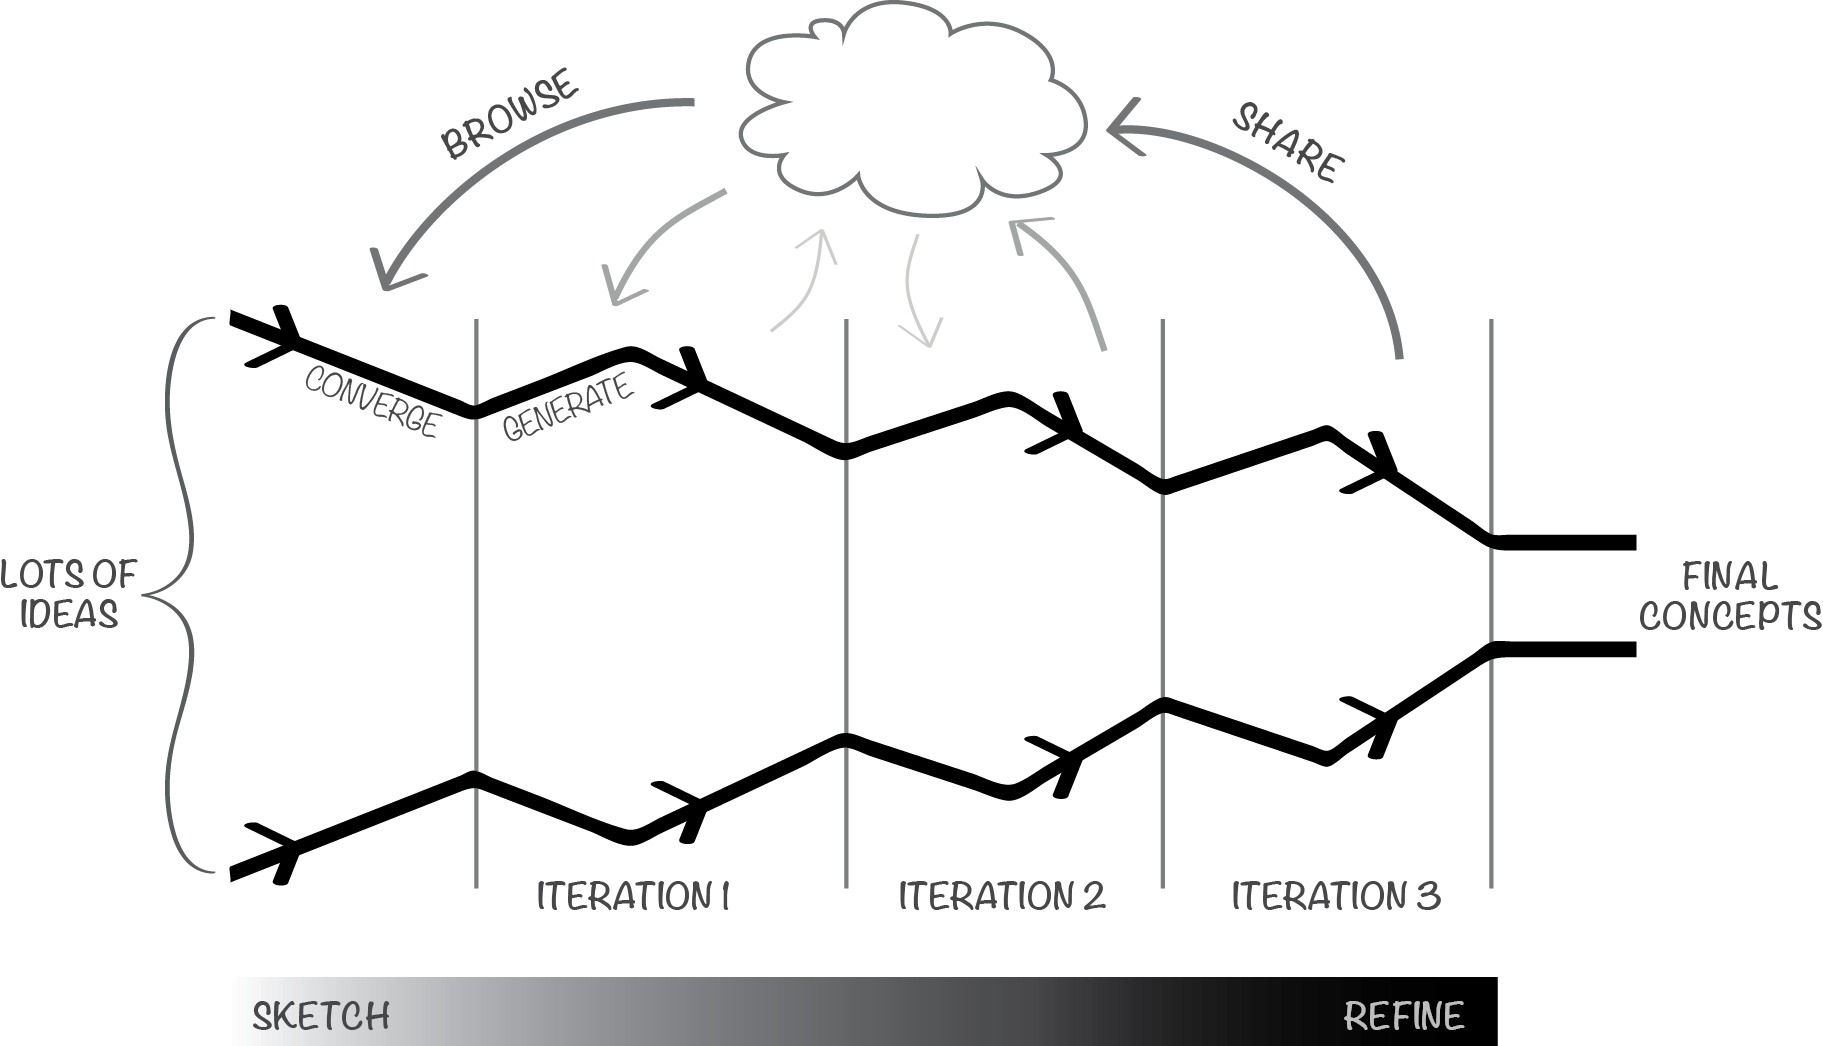
\includegraphics[width=\textwidth]{Fig1-4_Buxton-Adapted} 
   \caption{We found familiar design processes reflected in \haxd. We adapt the classic design funnel, where multiple initial ideas are iteratively developed~\cite{Buxton2007}, then add four design activities we have found useful when supporting design: \textit{browsing}, \textit{sketching}, \textit{refining} and \textit{sharing}. Exploring \haxd helped to reveal these activities, which are taken for granted in other fields but need to be explicitly supported for \haxd.}
   \label{fig:conclusion:buxtonaugmented}
\end{figure}


%
% SubSub - Browse
%
\subsubsection{Browse} 
``Browse" can have specific meanings for interacting with data (cite Munzner).
Here, we use ``Browse" to refer more generally to the act of looking at examples (\eg, corkboards of previous designs \cite{Buxton2007}, drawing from previous personal and professional experiences (\eg one's repertoire \cite{Schon1982} or real-life sources to inform a design.
We found this emerged in different ways:
in \autoref{ch:hapticinstrument}, participants used their personal experiences to interpret sensation meaning (\ie schemas, discussed more later);
in \autoref{ch:tactileanimation}, one animator brought up a YouTube video of a heartbeat to ground his animation;
in \autoref{ch:hapticianinterviews} several participants described collecting examples or using guide books.

We highlight this activity because haptic designers encounter modality-specific barriers when gathering, managing, and searching for examples.
Explicitly supporting browsing can make a difference:
in \autoref{ch:macaron}, we found visible, incorporable examples both eased design and helped scaffold learning for non-experts.
We believe scaffolding to be extremely important, as there are few haptic designers practicing today.
Browsing is also tightly associated with the ability to Share designs and collaborate; when one designer shares their designs or ideas, others are able to browse it.
We highlight three main challenges to supporting browsing in \haxd: representation, organization, and access.
%meanwhile, industrial designer Raymond Loewy espouses the need to balance the familiar and the new in design, creating the ``most advanced yet acceptable" design [].



%No idea is born in isolation.
%Individual designers have a repertoire of previous experiences they've encountered while learning or through practice~\cite{Schon1982}.
%In addition, design often starts with a ``gather" step~\cite{Warr2005}: viewing examples for inspiration and problem definition.
%Gathering often occurs explicitly at the start of a design process, and can reoccur during iteration.
%Tangible examples are corkboards and mood boards, which allow ideas to ``bake in" to the background~\cite{Buxton2007}.
%Software tools like d.tour~\cite{Ritchie2011} and Bricolage~\cite{Kumar2011} recommend websites for inspiration and can automatically generate new ideas by combining sites.
%\osC{make sure this doesn't overlap too much with Background}


 \inlineHeading{Representations of single sensations:} 
    How do we store, view, and organize haptic experiences?
    Haptic technologies are often inherently interactive, part of a multimodal experience with visual and audio feedback, and can take a variety of physical forms depending on the output (and input) device.
    This last point is particularly bothersome should the user not have access to the original device type -- imagine trying to browse force-feedback sensations on your phone!

\inlineHeading{Collection classification and organization:}
    Haptic language and cultures of meaning are still in active development.
    Without a commonly shared lexicon, organization dimensions, or even adjectives, it is difficult to curate collections.
    Compare this to sound: most musical terms have a long tradition with a clearly defined lexicon (\eg, crescendo, staccato); non-musical sound effects generally ``sound like'' something, and are often literal.
    With vision, one does not have to be a graphic designer or artist to instinctively understand ``warm" and ``cool" colours; the color wheel is introduced to us in grade school.  
    
   \inlineHeading{Overviews and skimming:} 
    Collections of examples, especially visual or physical collections, are often displayed spatially for ambient reference or to enable quick scanning.
    When you can't feel multiple things, it can be hard to get the big picture or swiftly peruse a collection.
    Both designer and end-users have needs for finding similar/different vibrations in a collection, requiring a low barrier-to-entry on any overview technique.
    \osC{also comment on search.}


%
% SubSub - Sketch
%
\subsubsection{Sketch}
Sketching allows people to form abstracted, partial views of a problem or design, iterate very rapidly and explore concepts.
The generalized notion of sketching can support other activities: sketches are a notation that can be shared, and provide a vehicle for annotating and iterating on designs.
Here, we use ``Sketch" in contrast with Refinement, to refer to embodied exploration, concept generation, and initial design.

Early in our exploration, we found that our Haptic Instrument, mHIVE, excelled for exploring a design space but faltered for refining sensations.
A real-time direct manipulation model in Tactile Animation facilitated both.
In Macaron, we observed different levels of exploration and refinement, discovering a pattern of focused adjustment and repeated reflection \cite{Schon1982}, where the designers stepped back to feel their design in its entirety, and zoomed in to adjust parts in detail.
We find this is a repeated pattern, where participants iteratively zoom in and out to different levels.
The mixture of focus also depended on the stage of design - early on, exploration and execution take a more prominent role, while later refinement has smaller adjustments and more reflection.
We have found this distinction useful when developing suites of tools, most explicitly when supporting design of CuddleBit behaviours.
Voodle is a free-form Sketching tool, which can hand off to MacaronBit for Refinement.
Future work remains to be done to establish whether there are discrete levels of focus, or if they lie along a continuum.
In general, we've found two main features important for supporting Sketching: \textit{abstraction and ambiguity}, and \textit{rapid iteration}.


%This is mostly heavily used early in design, and plays a role in collaboration (discussed more in ``Share'' below).
%Of course, such a central technique is used as a key way of thinking about experience design~\cite{Buxton2007}; 
%some even consider sketching to be the primary language of design, equivalent to mathematics as a language for natural sciences~\cite{Cross2006}.
%


\inlineHeading{Abstractability and ambiguity:}
	Haptics suffers from a dearth of notation.
	Sketching of physical devices or interfaces is well supported, with paper and pencil and innumerable software assists.
	Sketching \textit{motion}, and in particular showing what is or might be felt in, say, a vibrotactile experience, is  trickier.
	While we can sketch a visual interface and look at it, it is much harder to sketch a haptic sensation and imagine it without feeling it.

Creative approaches are emerging.
Most directly, \citet{Moussette2011} teach Haptic Sketching\footnote{\url{https://vimeo.com/29310105}} with physical scraps and materials, combined with manual actuator and tools like Arduino, to build effective interactive haptic prototypes physically and programmatically  in minutes or hours.
Simple display-only sensations can be sketched (\eg, VT icons)  using interactive design tools \cite{schneider2014improvising,Hong2013}.

\inlineHeading{Abstractability and ambiguity?:}

\inlineHeading{Sketching and Refining}
\osC{What about a planning/execution/reflection pattern?}



%
% SubSub - Refine
%
\subsubsection{Refine}
Clearly apparent in \autoref{fig:conclusion:buxton}, design requires iteration to refine an initial set of ideas into a single well-developed one through concept generation followed by iterative revision, problem-solving and  evaluation, until only small tweaks are necessary.
This long view of the design process is necessary to see designs through to the end;
further, tweaking final designs is a valuable way to accommodate individual differences, and was adopted by our haptic designers in \autoref{ch:hapticianinterviews}.

Incorporating haptic technology into a design is an extremely vertical process,  dependent on  specifics of hardware, firmware, software, application, and multimodal context.
With the complexity of these many components, there can be a significant initial cost to setup a first haptic experience; then, adding this complexity to the time needed to program, recompile, or download to a microcontroller means iteration cycles have the potential to be slow and painful. 
%
% Of course, there has been progress, and more is on the way. 
Thus, increasing refinement fluidity is ripe for innovation. For example:

\inlineHeading{Pipelines} now connect initial design seamlessly through to final refinement \cite{schneider2015tactile,Schneider2016macaron}.
Continuity in future tools will provide fluid, transparent (rather than cumbersome, many-staged) connection between hardware and software tools at different design stages.

\inlineHeading{Evaluation} is as crucial as for any human-centered refinement cycle. While it will often require some form of \textit{sharing} (coming up next), here we simply point out that the full spectrum of evaluative mechanisms and supports found in user experience development can be gainfully applied to haptic design, from lab-based comparative performance studies to qualitative examination of how usage strategies change when a physical dimension is deployed (\eg, \cite{minaker:2016:EH:handson}).

\inlineHeading{Customization tools} are appearing at least at level of prototyping and requirements generation \cite{SchneiderAsiaHaptics2014,Seifi2014}. 
Force-feedback virtual environments support iteration and refinement through code, once the initial environment is setup.
Software platforms like Unity\footnote{https://unity3d.com/} offer immediate control of variables in the UI itself.

\inlineHeading{Context} -- calibration, customization, and sensing -- in tools will help final haptic designs remain consistent depending on user activity (\eg, running impairs vibration sensitivity), individual differences, or other contextual concerns.

%
% SubSub - Share
%
\subsubsection{Share} 
Sharing designs is valuable at different stages of the design process \cite{Kulkarni2012}, whether for informal feedback from friends and colleagues, formal evaluation when refining designs, or distributing to the target audience for use and community for re-use \cite{Shneiderman2007}.

As haptic experiences must be felt, this process works best when collocated with only a few collaborators, whether by having collaborators work in the same lab, or by showing final experience in physical demos.
During ideation, ideas can be generated when collaborating remotely, but physical devices need to be shipped back and forth and it is difficult to troubleshoot and confirm that configuration and physical setup are the exact same.
Feedback also typically needs to be collocated, using in-lab studies or feedback, or shipping devices between collaborators.
Furthermore, visual and audio design support very easy capture of ideas to share later, through smartphone cameras and microphones, that could later be browsed.

So far, haptic broadcasting, analogous to broadcasting radio or television (\eg, Touch TV \cite{Modhrain2001}) has been envisioned and explored.
Followup work has added haptics to YouTube \cite{AbdurRahman2010} and movies \cite{Kim2009}.
Low-cost devices like the HapKit \cite{Martinez2016}\footnote{\url{http://hapkit.stanford.edu/}} and Haply \cite{Gallacher2016}\footnote{\url{http://www.haply.co}} make haptics more ubiquitous, but remain troublesome to calibrate.
To share ideas remotely on phones, proxies like visualizations or other types of haptics (phone vibrations) could be used \cite{Schneider2016b}\footnote{\url{http://www.cs.ubc.ca/labs/spin/hapturk}}.
Features like automatic calibration and proxies for use in online evaluation, and online communities more generally, are still in development.




%%%%%%%%%%%%%%%%%%
% SubSection - Paradigms and Representations
%%%%%%%%%%%%%%%%%%
\subsection{Generalizing Devices and Sensations}
One major challenge facing haptic designers is the variety of haptic devices available.
Each device has different physical properties, and may use different actuation principles or sensory modalities to communicate with the user.
This might be analogous to how modern web sites employ responsive design, adapting to different screen sizes, albeit more extreme.
A screen, at the end of the day, is that plane with a given physical size and pixel size; with haptics,
contextual problems like grip can influence feedback, and haptic feedback can vary from single VT actuators to VT grids, programmable friction, skin stretch, or force-feedback devices.
We suggest three ways of managing this complexity:
Grouping devices and interactions into \emph{paradigms},
considering representational \emph{translations}, and
using affordances and closed-loop sensing to create \emph{consistency}.
A fourth related strategy, enabling customization, is so important we discuss it later.


\subsubsection{Paradigms}
However, we believe this problem is more diverse than screen size and resolution.
We suggest this is a single \emph{paradigm} for graphic designers, analogous to how haptic designers might work with several different types of single vibrotactile actuators.
Haptic design becomes more diverse when designers need to consider arrays of VT actuators, programmable friction, skin stretch, or force-feedback, all of which are as analogous as screens are to, e.g., speakers.

First captured in Chapter \ref{ch:hapticianinterviews}, we believe that paradigms is a key concept to designing \haxd tools.
We define a ``paradigm" as an abstracted model of how to work (?) with a haptic device.
Much like how different programming language paradigms, such as functional or object-oriented languages, can accomplish similar results but enable programmers to think in different ways more appropriate to their problem, we believe that different haptic or multimodal paradigms will enable different problem solving techniques for \haxd.
In our in-depth studies we present three: an instrument paradigm, an animation paradigm, and a track-based editing paradigm.

It is critical to note that there is a many-to-many mapping between paradigms and haptic devices.
Tactile animation can be used for multiple spatial grids and track based editors are generalized enough to handle multiple display types.
Meanwhile, a multi-VT grid could be controlled by any of these three paradigms.
As haptic displays become more diverse, we expect paradigms to play a larger role for organizing design perspectives, and multi-paradigm tools to become successful, just as multi-paradigm programming languages like Python and JavaScript afford flexibility, power, and accessibility - providing increasingly low barriers, wide walls, and high ceilings.

\osC{Paradigms can be split into temporal, spatial, and interactive (reactive) elements.}

\subsubsection{Representation and Native Platform}
One striking problem with haptic technology is its sheer diversity.
There are a wide diversity of devices, many of which support different paradigms, and all of which can be different based on their physical configuration.
This poses a problem of access - if a designer creates a force-feedback sensation, how do you render that on a mobile device with a simple vibrotactile actuator?
Can this translation be done?

Compare this to graphic design.
At the end of the day, most graphic designs will be on a 2D plane, whether a screen or not.
There are different sizes, resolutions, and colour maps - for example, print media might be designed differently than web - but similar tools and principles apply.
In haptics, we might apply these different sizes and resolutions to a class of device - for example, a VT actuator can be an expensive C2 tactor or a low-cost voice coil.
However, a single actuator is quite different from a 2D grid of actuators (like in Tactile Animation), and dramatically different from variable friction feedback (like with Rough Sketch) or 1-DoF force feedback (like with HandsOn).
The question of resolution and platform within a single class of devices is analogous to the challenges faced by graphic designers and sound designers, but the diversity of classes of devices is even more varied.

\subsubsection{Consistency through sensors and context control}
A third way to adapt to the variety of contexts a haptic device might be used in is to either impose a known context, or sense and adapt an uncontrollable context.

Our industry haptic designers would talk about working with automotive companies, and how the material in the dashboard could affect the final haptic sensation.
By controlling this material and working in a known environment, haptic designers might be able to keep their designs more consistent:
When actuating a touch-screen in a car, a designer could know the materials.
Similarly, wearable devices like the wristbands (Pebble, Apple Watch) know where the device will be worn, and can use that knowledge to their advantage; they can also use the materials of their wrist-straps to ensure a reliable tightness or pressure on the skin.
Force-feedback devices like haptic knobs might change their handles, using physical affordances (Gibson? Norman?) to suggest a grip to the user.

Alternatively, closed-loop sensing might be able to standardize sensations.
\citet{Blum2015} showed that accelerometers can provide insight into perceived loudness of VT stimuli.
Techniques like activity classification (\eg \cite{Schneider2013}), or even vibration sensing of a VT effect could help reduce noise from physical changes and material properties.
This could be done \emph{in-situ}, or during manufacturing for different device materials as a quality assurance step.

%%%%%%%%%%%%%%%%%%
%
% Section - Meaning
%
%%%%%%%%%%%%%%%%%%
\subsection{Designing Meaning}
Because of the novelty of haptic design, we found that conceptual schemas are important for understanding the intent of haptic sensations.
Schemas are existing conceptual models used as transitionary objects to understanding new concepts \cite{Papert1980}.
We found this procedure occurred not only in educational contexts, but also in design.
In our early Haptic Instrument exploration, we found our participants' prior experience was a lens through which they interpreted haptic sensations.
For example, one cat-owning participant interpreted likened sensations to cat purring, while another drew more on their knowledge of engines and cars.
Heartbeats and rain \cite{Israr2014} are effects that were easily understand by general participants, and verified using perceptual studies.
Schemas are useful both for framing user interpretation of haptic experiences, and for designers themselves.
We have also found the concept of design languages and narrative as helpful ideas when creating experiences.

\subsubsection{Schemas as a tool for users}
To interpret haptic signals, people employ a number of conceptual or translational  schemas, often combining them.  % frameworks
We might compare a haptic sensation to a natural one (``This is like a cat purring''), 
 to emotions and feelings (``This is boring'''), or
consider its potential usage (when a quickening tactile pulse sequence is described as a ``speed up''). 
%
The meaning someone chooses is typically influenced by the sensation itself but also by the context of use and the user's background and past experiences~\cite{seifi2015vibviz, schneider2014improvising, Obrist2013}. 

%\begin{figure}[bt]
%        \centering
%        \includegraphics[height=2.5in]{figures/InterpretiveFacets3}
%        \caption{People use a variety of cognitive frameworks to make sense of haptic signals.}
%        \label{fig:interpSchemas}
%    \end{figure}
    
\textit{Facets} are a concept originating from the domain of library and information retrieval which nicely capture the multiplicity and flexibility of users' sense-making schemas for haptic sensations. A facet is a set of related properties or labels that describe an aspect of an object~\cite{facetedbrowsing2010}. Five descriptive facets have been proposed and examined for haptic vibrotactile stimuli \cite{seifi2015vibviz}: physical properties, sensory properties, emotional connotations, metaphors, and usage examples.
 
%    \textit{\textbf{Physical}} properties that can be measured -- such as duration, energy
%    
%    \textit{\textbf{Sensory}} properties -- roughness, softness
%    
%    \textit{\textbf{Emotional}} connotations -- pleasantness, urgency 
%        
%    \textit{\textbf{Metaphors}} or familiar examples to describe a vibration's feel -- drumbeat, cat purring
%    
%    \textit{\textbf{Usage examples}} or types of events where a vibration fits -- ``speed up'', ``time's up''

If a designer neglects a consistent consideration of these meaning assignment facets % frameworks, 
the result is likely to be confusion and bad user experience.
Leveraged properly, facet-driven 
mappings can be lead to more intuitive, consistent results and highlight pathways to work around individual differences, for example through tools that allow users to efficiently customize their interfaces.

Schemas can also be used for haptic designers to help frame their design processes.
As covered in \autoref{ch:rw}, many previous systems have their roots in other, non-haptic concepts, \eg Touch TV \cite{}.
This enables transfer effects; as we showed with Tactile Animation (\autoref{ch:tactileanimation}), visual animators were able to easily create tactile designs.

\subsubsection{Design Languages}
Another way of framing a haptic experience is to use a \emph{design language} like Google's Material Design (\url{https://material.google.com}).
A design language is a defined set of aesthetic and interactive rules to ensure a consistent look-and-feel.
We also believe that Gestalt-like principles will play a role in defining the possible design languages for haptics,
much like musical concepts of thematic development, restatement, elaboration, and expectation, or graphical design concepts like contrast, repetition, alignment, and proximity are the tool with which languages can be formed.
Previous efforts have identified frequency, amplitude, rhythm, affect, and spatial location as the main design elements for vibrotactile design.
We have started to identify similar, middle level concepts - alignment and repetition emerged in the Macaron study.


\subsubsection{Narrative Context and Multimodal Reinforcement}
The intent of a haptic sensation was not always interpretable from the sensation itself.
A great deal of the interpretation of an effect depended on the narrative context.
Previous work used linguistic descriptions, such as ``light rain" \cite{Israr2014}.
In our FeelCraft and Feel Messenger studies, we found that linking adaptable sensations to in-game stimuli was effective.
With Feel Messenger, we at first attempted feel effects with abstract icons, such as ``motor" for a rumble effect. 
In early piloting, these were not very helpful for understanding.
Adding in vibrant cartoon emoji icons, and using  a cat's face (for a purr) rather than a motor image were much more effective in sending haptic icons.

It is also worth mentioning the role of realism in a haptic experience.
There are two types of realism, photo-realism (veridicality) and real-seeming (verisimillitude) (cite McCloud).
For example, cartoons and animation are clearly not depictions of reality (they do not display veridicality), but they can appear life-like (they display verisimilitude).
In this dissertation, we focused on verisimillitude rather than veridicality; the latter is often already accommodated by realistic rendering techniques.
We believe both require a design process, but more photo-realistic approaches have different challenges than cartoony ones, and may require more of an engineering perspective than a design perspective.
That said, sometimes combining the two is helpful; much like how in computer graphics, physical simulation and realistic rendering are used as a baseline, but artists still may want artistic control over certain scenes or effects.




%%%%%%%%%%%%%%%%%%
% SubSection - Customization
%%%%%%%%%%%%%%%%%%
\subsection{Customization}
We've shown how individual differences are a prominent feature of haptic perception and psychology.
Furthermore,  variability in and poor designer control over context --  user attention and  device form factor and manner of connection, as well as use environment -- mean that haptic sensations often need to be tuned to both each person and each use case.

The most likely solution   is to make it easy for end-users in populations that might benefit from a haptic modality to \textit{customize} aspects of haptic design elements, whether by choosing pre-formed settings and ``skins'', adapting defaults, or wholly designing their own. 
Possible approaches range from volume-like slider controls, options to select sensations from curated collections, or, at the more complex end, perceptually-confirmed filters like those found in Instagram or PhotoShop~\cite{Seifi2014,seifi2015vibviz,SchneiderAsiaHaptics2014}.


\inlineHeading{Volume Controls}
As found in our interviews with designers, the end-user context is sometimes unknowable.
There is not much designers can do other than putting a volume control on their design to facillitate customization.
In informal discussions with engineers from commercial companies (\eg D-Box), volume controls were a critical, early addition to their haptic chairs.
As explored in our FeelCraft and FeelChat projects, the extra level of volume control is implementable, expressive, reduces footprints, but is more limiting for designers and requires programming expertise.
While there is a great deal of noise in perceptual parameters for high-level controls, careful investigation can improve this \cite{Israr2014,Seifi2014}.



\inlineHeading{Novelty and Irritation}
Haptic sensations are new, giving them great power and great responsibility.
They can grab attention, but designers must take care not to annoy with constant haptic feedback.
The balance is tricky. 
Good design might be not even noticed when present.
With RoughSketch, we found that allowing a button to remove haptic feedback was very persuasive for appropriate, non-irritating designs.
We also found that muting features were essential for \haxd design tools.






\section{\haxd Tools: Designing and Implementing}
In this section, we comment on the specific features and forms \haxd support tools might involve.
Because of the diverse activities described in the previous section, we believe there is no silver bullet: haptic design tools are likely to form a suite or ecosystem.
Here, we discuss ways to enable creativity through mature tools with ``a low barrier, wide walls, and a high ceiling."
We talk about important collaborative techniques and how to deploy implemented tools.
We discuss implications for developers and software engineering teams.
Finally, we conclude with some comments on our evaluation methodology and how future \haxd tools might be evaluated.


%%%%%%%%%%%%%%%%%%
% SubSection - Online Communities
%%%%%%%%%%%%%%%%%%
\subsection{Communities and On-line Deployment}
Unfortunately, haptic technology faces obstacles to Browsing and Sharing, especially when under development; this has typically confined distribution and exposure to lab prototypes available only to in-person visitors.
Demos are difficult to setup and there is little infrastructure in place for distribution.
While synchronous, collocated collaboration is effective with demos, remote or asynchronous collaboration is rife with trouble.
Consistency must be maintained, and setup can be painful for those not trained in setting up devices.
On top of this, we found a strong tendency to show, not tell sensations, and an impoverished language especially for non-experts.
Without a shared reference point of physically feeling the sensation, we believe that design can be easier, especially when a language of design is underdeveloped.

Recently, online interfaces have emerged for sourcing content, distributing content, and distributing media itself. 
We found that moving to a web-based tool with Macaron greatly facillitated distribution.
Online deployment simultaneously widens exposure and speeds development, making it easier for designers to be inspired by or directly build upon one another's work. 
The trend will accelerate as the field matures, but there will need to be concurrent development of accessible hardware to connect with software tools.

\subsubsection{Crowdsourcing and broadcasting:} 
    We reviewed some of the substantial challenges and spoke of one type of solution.
    In HapTurk (\autoref{ch:hapturk}), we showed proxies of high quality haptic experiences  can communicate key aspects on more shareable media, to gain access to crowdsource evaluation tools like Mechanical Turk.
    Proxies might be able to generalize in other ways, for example, using video to infer feedback about physically moving objects like the CuddleBits (\eg as in \cite{Pedersen2014}).

    Proxies can do more than elicit feedback from crowds.
    It might also be a viable way to translate sensations between representations, analogous to downsampling high-definition video broadcasts for standard definition televisions.
    More exotic proxies, like using vibrotactile feedback to represent force or friction could be considered. 
    Future perceptual studies are needed to accomplish this.
    
\subsubsection{Open Haptics -- design sharing communities:} 
    % While remote engagement can introduce other issues, they not only provide corresponding benefits but also can be complementary to existing practices. 
    Other kinds of designer-facing online communities and outreach activities may assist with open haptic media -- making it easier to share design resources,  build up a haptics design culture, and, where possible, cooperate on establishing a consistent design language of haptics. 
%
    For example, online software like VibViz~\cite{seifi2015vibviz} and Macaron~(\autoref{ch:macaron}) provide details to designers anywhere, while open hardware projects like HapKit~\cite{Martinez2016} and Haply~\cite{Gallacher2016} are available to hackers and students.
    Conference workshops and hardware kits provide users and designers with additional means to experiment with advanced haptics.
    
    Each of these projects solve different problems and provide independent benefits.
    Online collaboration, and resources like articles on haptic perception or tutorials on how to effectively create haptics, will connect more designers, artists, developers, students, and hackers and help to build haptics into new user experiences.


\subsubsection{Examples, demos, Show, don't tell}
We found that demonstrations were critical for haptic designers in the wild.
To help elicit requirements, customers were brought in to try out various demos.
To persuade customers, actually feeling the haptics was critical, if not always enough.
The Haptic Instrument showed evidence for deictic features - what do you think of ``this", which facillitated direct demonstration without having to resort to indirect linguistic descriptions.
In Macaron, exposing the underlying structure of examples lead to improved understanding of how to develop sensations and developed haptic idioms.





\inlineHeading{Risk}
Adding haptics is risky.
\osC{we say this quite well in the previous 8.4 discussion, why should we repeat it?}




%%%%%%%%%%%%%%%%%%
%
% Section - Towards Mature Tool Suite
%
%%%%%%%%%%%%%%%%%%
\subsection{Towards a Mature \haxd Tool Suite}


%%%%%%%%%%%%%%%%%%
% SubSection - Examples
%%%%%%%%%%%%%%%%%%

\inlineHeading{Soft Features}
Repeatedly, participants asked for ``soft features", associated with more polished tools.
This includes features like copy and paste, undo and redo, saving and loading, grouping, looping, reduced delay, and high-fidelity rendering.
We increasingly found, as we iteratively developed \haxd tools, that these features are more important than getting the right paradigm.
As long as a designer is able to freely and accurately create, they can work around awkward design metaphors.

\inlineHeading{Low barrier, wide walls, high ceiling}
A major goal of our work was to support creativity with haptic technology, and to support low barriers, wide walls, and a high ceiling \cite{Shneiderman2007,Resnick2008}.
We've confirmed that this is critical for \haxd, and found ways of accomplishing it.
As we mentioned, our participants found soft features essential, which helped to free them to make mistakes, explore various options, and provide both accessibility (low barriers) and refinement (high ceilings).
For example, in Tactile Animation, participants found the animation objects easier for exploration and non-expert designers, while vector sensations offered more fine-tuned control.
Similarly, we found the more flexible track-based paradigm used by Macaron to allow for various paths through the interface, and was generalizable to other sensations like simple 1-DOF robots.



Making haptics means different things at different stages in the process (Section~\ref{sec:4:Making}). 
Media creation in other modalities is supported with a wealth of tool specializations that recognize these diverse needs. Haptic making has reached a maturity that demands tool power, nuance, and specialization as well.

Some of the important ground to cover here includes better support for \textit{sketching}, \textit{high-level manipulations}, \textit{multimodal qualitative analysis} and \textit{browsing}, as well as workflow integration and addition of specific useful features to tools that already do exist.

%
% SubSub - Sketching
%
\subsubsection{Allowing Sketchiness}
Early design needs support for low-cost, rapid ideation that elevates key points without extraneous detail. Haptic design presents a few challenges; solving these will further empower designers.

\textit{Ambiguous sketches} show only necessary detail or relevant view points, helping a designer work with half-formed ideas and questions, but a haptic sensation requires a physical implementation which must be exactly specified. 
%
We need to explore different approaches to quick prototyping of different haptic aspects -- \eg, feel, form factor, timing. One approach is \textit{modularity}: prototyping one aspect at a time, then integrating into more expensive engineering prototypes once the design space has been narrowed. Here, the tool need is both for ready-to-go platforms to explore single-aspect ideas, and ways to efficiently extract, port, or integrate best-of-breed sketches into later design stages.
    
\inlineHeading{Good defaults:} In another approach, designers will be able to select from carefully chosen default settings, and/or specify  any known constraints with other details be filled in automatically. 
    
\inlineHeading{Annotation:} Sketching should supply markup support for both early-stage designers themselves and the stakeholders they share with, to  annotate sketches, circle problem areas, and write down related ideas.
    
\inlineHeading{Ad-hoc use:} Finally, tools should be easy to access. With a pen, any napkin is a canvas. Haptics (and multimodal interactions in general) need napkins too. 


%
% SubSub - Low-level
%
\subsubsection{Fluid control of low-level parameters}
A viable approach enabled by our real-time tools is an implicit understanding of the sensations by designers, who were able to work with low-level engineering parameters like frequency, amplitude, or even voltage.
In the Tactile Animation study, we found that while animation objects were more used and described are more accessible for non-animators, vector sensations (directly controlling each actuator) were described as useful for finer, expert control.
Learning to control low-level parameters is important for ``high ceilings" in \haxd support tools.



%
% SubSub - High-level
%
\subsubsection{High-Level Manipulations} 
The haptics community currently has access to a number of editing tools which together exhibit a variety of approaches to editing and authoring, primarily of low level effect detail (Section~\ref{sec:make_tools}).
However, being able to manipulate sensations in the large or in an expressive way will enable designers to access a larger design space, and do more in less time.

In other modalities (Photoshop for graphic media, Audacity for sound), this kind of functionality appears in a variety of ways.  
\textit{Filters} are essentially ``tuners'' that move a sensation along dimensions of direct design interest.
\textit{Transformations} allow users to alter or distort a segment, \eg, to darken or brighten it,  stretch its time base in a linear or nonlinear way, or shift component balance.
%
\textit{Large-scale manipulations} can move, combine, subtract and otherwise alter design elements.

The scope of such manipulations should span perceptual, informational, and affective perspectives. Research is underway to understanding these manipulations from user perceptual and subjective standpoints, and implement them algorithmically. 


%
% SubSub - Engineering features into mature tools
%
\subsubsection{Engineering useful features into mature tools} 
Both individual experiences in designing with haptics, and reference to tools in other modalities show the value of seamless access to many small but useful features --
direct manipulation, undo/redo, copy/paste, selection and group manipulation, import/export to various formats, access to a library, etc..
%
Individually, many of these do not present major research or usability problems, but integrating them is another matter. There are at least two obvious approaches:

\inlineHeading{Additive:} 
    Haptics authoring capability can be added to existing mature platforms focused on another modality -- \eg, to Photoshop (for graphics)  or Premier (video).
    Force-feedback is already integrable into certain video game and virtual world environments (Unity, XNA), but this is only a small subset of possible haptic experiences.

\inlineHeading{Haptics-specific:} 
    To truly optimize haptics capabilities, it may be worthwhile to invest serious development into a haptics-specific platform; or more likely, many attempts at such a thing focused on different categories of hardware (\eg, tactile wearables versus 3D desktop force feedback environments) or application area, perhaps by extending initial low-level editors already available.

\vspace{0.1in} \noindent 
Researchers are good at pioneering individual steps and features, but integration is a significant development initiative which lies more in the province of businesses who stand to profit by the effort invested. 
Which task focus and development pipelines are to be supported, including multimodal design and integration,  will be driven by application areas with urgent needs and a promising economic prognosis:  \eg, for movie special effects versus surgical simulations or end-user customizations.


%
% SubSub - Engineering features into mature tools
%
\subsubsection{Iteration}
In our interviews, we found iteration was extremely painful.
Despite this, we've found iteration is necessary (as with all design processes), but even more so because it is difficult to understand requirements or identify a good design without feeling it.
Many of our designers would iterate until it ``felt right".
Thus, iteration is very necessary yet very painful.




%%%%%%%%%%%%%%%%%%
%
% Section - Implementation
%
%%%%%%%%%%%%%%%%%%
\subsection{Notes on Implementing \haxd Tools}
During our in-depth studies, we looked at three different platforms for implementing \haxd support tools: Android on tablet for mHIVE, Python on desktop for Mango, and JavaScript deployed on the web for Macaron.
From these three implementations, and from attempting to distribute or deploy them, we have found several lessons for implementing interactive software for \haxd support.
Many of these are straightforward applications of software engineering, but we particularly found recently developed web tools to be especially useful when managing the complex interfaces required by design tools.

\inlineHeading{Observer Pattern}
Well established as a design pattern \cite{}, the found the observer pattern was critical in keeping the complex interfaces of our design tools synchronized.
This is especially critical because we need to synchronize haptic, audio, and video playback, and allow implementations through both temporal and spatial means.
In Mango, we implemented this pattern ourselves, but in Macaron, we used React \cite{} which automates the process.
This latter approach was more efficient and facillitated programming.

\inlineHeading{Components and Track-based Editing}
Another valuable approach to develop extensible tools was React's Components, composable interface elements that can be parameterized and reused.
This technique, along with a carefully organized architecture and the generic track-based editor control paradigm used by Macaron made it very easy to extend.
When developing MacaronBit by forking the original code for Macaron, we were able to repurpose the tool to control the CuddleBits in a single day.
While a better paradigm could be designed, our in-lab experts were able to used generalized tracks to create differentiable behaviours from the bit.
One can also imagine redesigning a track-based editor to use a different control paradigm with the same device - we do this with MacaronMix, which mixes two VT icons using again a fork off of Macaron.


\inlineHeading{Flexible, extensible data structures}
Because of the complexity and variance of haptic devices, we needed to establish data structures that were lightweight but extensible.
We used JavaScript Object Notation (JSON) to accomplish this in Mango, Macaron, and FeelCraft.
JSON which allowed us to specify only the required information needed, whether for device parameters in Mango, or sensations created by both Mango and Macaron.
Our tools would check JSON files for designed features - like amplitude tracks in Mango - and ignore others we left in for a stub - like frequency tracks.
These structures were simple, human-readable, ignored extraneous detail, and could gracefully fail when poorly formatted.
Because we need to accommodate different paradigms in \haxd tools, lightweight data types make a lot of sense.

\inlineHeading{Existing data structures like .WAV}
Audio control useful, Arduino connection useful - but how to connect to web?


\inlineHeading{Web Deployment}
One challenge with haptic technology 
Web - more people, online communities, resources, show internal structure
Need to package up software
Documentation for use

\inlineHeading{No Delay}
In interviews with designers, we found that delay was critical; multimodal sensations had to be tightly synchronized.
We found similar problems with our tools.
mHIVE had a short delay which was distracting to participants, particularly when they tried to play very short pulses.
Macaron's real-time audio synthesizer sometimes created a ``muddy" effect (P?) because it had a limited update rate.
We found this disappeared after implemented .WAV exporting function.
Combined with our findings that users would switch between focused, in-depth editing and more reflective experiencing, we suggest (and are working to implement) a pre-feel/render model, like with visual effects tools.
This is one potential problem with current web implementations of our design tools, especially when attempting to communicate to embodied devices like Arduino.


\inlineHeading{Distribution requires hardware}
An obvious, but critical, requirement for \haxd tools is that they require the appropriate hardware.
Above we've discussed flexible architectures and data structures to support different hardwares and paradigms of sensations.
In addition, potential designers need easy access to hardware.
One way we've found is to create do-it-yourself haptic wristbands for Macaron. (URL)
Critical for VT feedback is that amplifiers and actuators matter - we found the DIY custom amplifier we've built does not have the same crispness as a more expensive commercial audio amplifier.
This means that modular systems could be designed for facillitate accessible haptic feedback and design, but are complicated in because the setup doesn't end at the actuator.
Another approach is to use a HapTurk-based translation with mobile vibrations like those available on Android (link to hapticJS), although this impoverishes sensations and leads to the challenge of native platform, discussed above.


\inlineHeading{Logging and Analytics}
One important feature for modern software is remote analytics.
Various types of metrics and usage statistics help developers prioritize development, fix bugs, and report to investors.
Interestingly, because haptic technology extends into the physical world, one can consider using remote analytics both on their design and playback software, and on the physical devices.
With a modular system
Logging and analytics not a problem; should record these features (from Macaron, a little Tactile Animation)




%%%%%%%%%%%%%%%%%%
%
% Section - Evaluation
%
%%%%%%%%%%%%%%%%%%
\subsection{Evaluating \haxd Tools}


%%%%%%%%%%%%%%%%%%
% SubSection - Flow, learning, scaffolding
%%%%%%%%%%%%%%%%%%
\subsubsection{Flow, Learning, Scaffolding, and Embodiment}




\subsubsection{Exploratory Analysis and Visualization Tools (Haptic Analytics)} 
Haptic researchers frequently analyze haptic datasets with the goal of informing next steps in a design use case or deriving design guidelines for the haptic community. 
Such an  investigation usually involves exploratory analysis of quantitative and qualitative attributes of signals and users' perceptions. 
Currently, designers use a potpourri of general-purpose software (\eg, Matlab, R, SPSS, Tableau) for their analysis. Each tool provides just a partial view of the data; the difficutly of integrating their insights hinders the analysis process. 

Visual analytics interfaces, which support analytical reasoning through interactive visualization of datasets, are largely absent from haptics at this time. 
Examples of desirable functionalities  include easy access to the feel and source of signals, enabling rapid and flexible organization of haptic signals according to their various properties, allowing researchers (and the crowd) to attach metadata (tags, genealogy, annotations) to elements and subsets of a haptic collection, and do analytics on this metadata.


The first steps towards haptic analytic interfaces (Section~\ref{sec:make_tools}) have exposed some of the work that's needed to make these truly useful. Much of it is the same underlying perceptual knowledge and  algorithmic advances required for authoring and manipulation, \eg, of perceptual dimensions and user's mental organization and ways of differentiating and interpreting sensations, and this is well underway. 
%
Connection to or integration of multimodal functionality -- \eg, suitability for coordinating with design elements from other modalities, in various communication roles (Section~\ref{sec:IM_roles}) -- will develop along with our experience in working with these modalities. 



\inlineHeading{Post interviews}
Early in our investigation, we found that participants found traditional think-aloud [] protocols challenging.
This appeared to be due to a split attention of paying close attention to sensory input on their hand while simultaneously designing sensations.
Even without thinking-aloud, this was cognitively challenging, and participants wanted looping, or would step back to refine and feel their sensations.
In response, we adopted unintrusive logging and post-interviews, both of which were effective in capturing aspects of the haptic design process. 

\inlineHeading{Phenomenology}
Because of the close connection with participant experience, we adopted techniques from phenomenology, both to capture the sensory experience of haptic sensations, and to capture the experience of design.
This perspective was useful for rigorous examination of our participants' interviews and to guide the interview process.
In addition, the practical techniques, considering each meaning unit and clustering them into both in-vivo language and analytical language, very useful, especially when later combined with Grounded Theory techniques.

\inlineHeading{Grounded Theory}
To better equip ourselves to analyze larger sets of data and develop a broader theory, we also drew upon Grounded Theory as described by Corbin and Strauss [].
Especially when analyzing screen-captured video, coding techniques were valuable in identifying countable data, strategies, and adding a second layer of data analysis techniques to complement those provided by phenomenology.

\inlineHeading{Analytics and Logs}
Qualitative analysis of post-interviews provided valuable insight, but only gave a partial view of haptic experience design.
Timing analysis, and visualized logs, captured data that may not have been not have been observed by the researcher, and not reported or noticed by the participant in a post-interview.
Importantly, it also offers a transition into broader data collection at large, providing a sustainable method of observing features


\inlineHeading{Multimodal Design Tasks}
Throughout our three in-depth design tool studies, we refined our approach for participant tasks.
With the initial Haptic Instrument study, we asked participants to freely explore the interface and attempt to design for affective words like happy or sad.
This was challenging for the participants, and we found inconsistent designs. \osC{TODO: what exactly was bad about this?}
In our Tactile Animation study, we used more defined scenarios - a heartbeat, a directional cue for driving, and a sound-based design task.
The first two were effective and descriptive for our participants, but the sound task in particular engaged them; it also gave us controls over theoretical dimensions like complexity or abstractness, impose constraints like careful timing, and was externally valid with the multimodal nature of haptic design.
In our final in-depth study, we adopted animations instead of sounds, with similar results.

\inlineHeading{Ratings}
In our studies, we had participants rate their designs including confidence and difficulty.
We did not find quantitative results from these reports, mostly due to low sample size and the qualitative nature of analysis.
However, we did find it to be useful for two reasons.
First, it provided an elicitation device, inviting participants to comment on the difficulty or their happiness with their designs.
Second, as we scale to more natural settings and higher sample sizes, we hope quantitative findings from rating scales will provide insight to questions about challenge, learning, and flow theory, which emerged from the third in-depth study.




%%%%%%%%%%%%%%%%%%
%
% Section - Future Work
%
%%%%%%%%%%%%%%%%%%
\section{Current and Future Work}
\osC{todo}



%%%%%%%%%%%%%%%%%%
%
% Section - Conclusion
%
%%%%%%%%%%%%%%%%%%
\section{Conclusion}
\osC{todo}




%%%%%%%%%%%%%%%%%%%%%%%%%%%%%%%%%%%%%%%%%%%%%%%%%%%%%%%%%%%%%%%%%%%%%%%%%
%%%%%%%%%%%%%%%%%%%%%%%%%%%%%%%%%%%%%%%%%%%%%%%%%%%%%%%%%%%%%%%%%%%%%%%%%
%%%%%%%%%%%%%%%%%%%%%%%%%%%%%%%%%%%%%%%%%%%%%%%%%%%%%%%%%%%%%%%%%%%%%%%%%
%%%%%%%%%%%%%%%%%%%%%%%%%%%%%%%%%%%%%%%%%%%%%%%%%%%%%%%%%%%%%%%%%%%%%%%%%
%%%%%%%%%%%%%%%						MAJOR SECTION BREAK						%%%%%%%%%%%%%%%
%%%%%%%%%%%%%%%%%%%%%%%%%%%%%%%%%%%%%%%%%%%%%%%%%%%%%%%%%%%%%%%%%%%%%%%%%
%%%%%%%%%%%%%%%%%%%%%%%%%%%%%%%%%%%%%%%%%%%%%%%%%%%%%%%%%%%%%%%%%%%%%%%%%
%%%%%%%%%%%%%%%%%%%%%%%%%%%%%%%%%%%%%%%%%%%%%%%%%%%%%%%%%%%%%%%%%%%%%%%%%
%%%%%%%%%%%%%%%%%%%%%%%%%%%%%%%%%%%%%%%%%%%%%%%%%%%%%%%%%%%%%%%%%%%%%%%%%

\section{Previous HaXD theory}


\begin{figure}[h] %  figure placement: here, top, bottom, or page
   \centering
   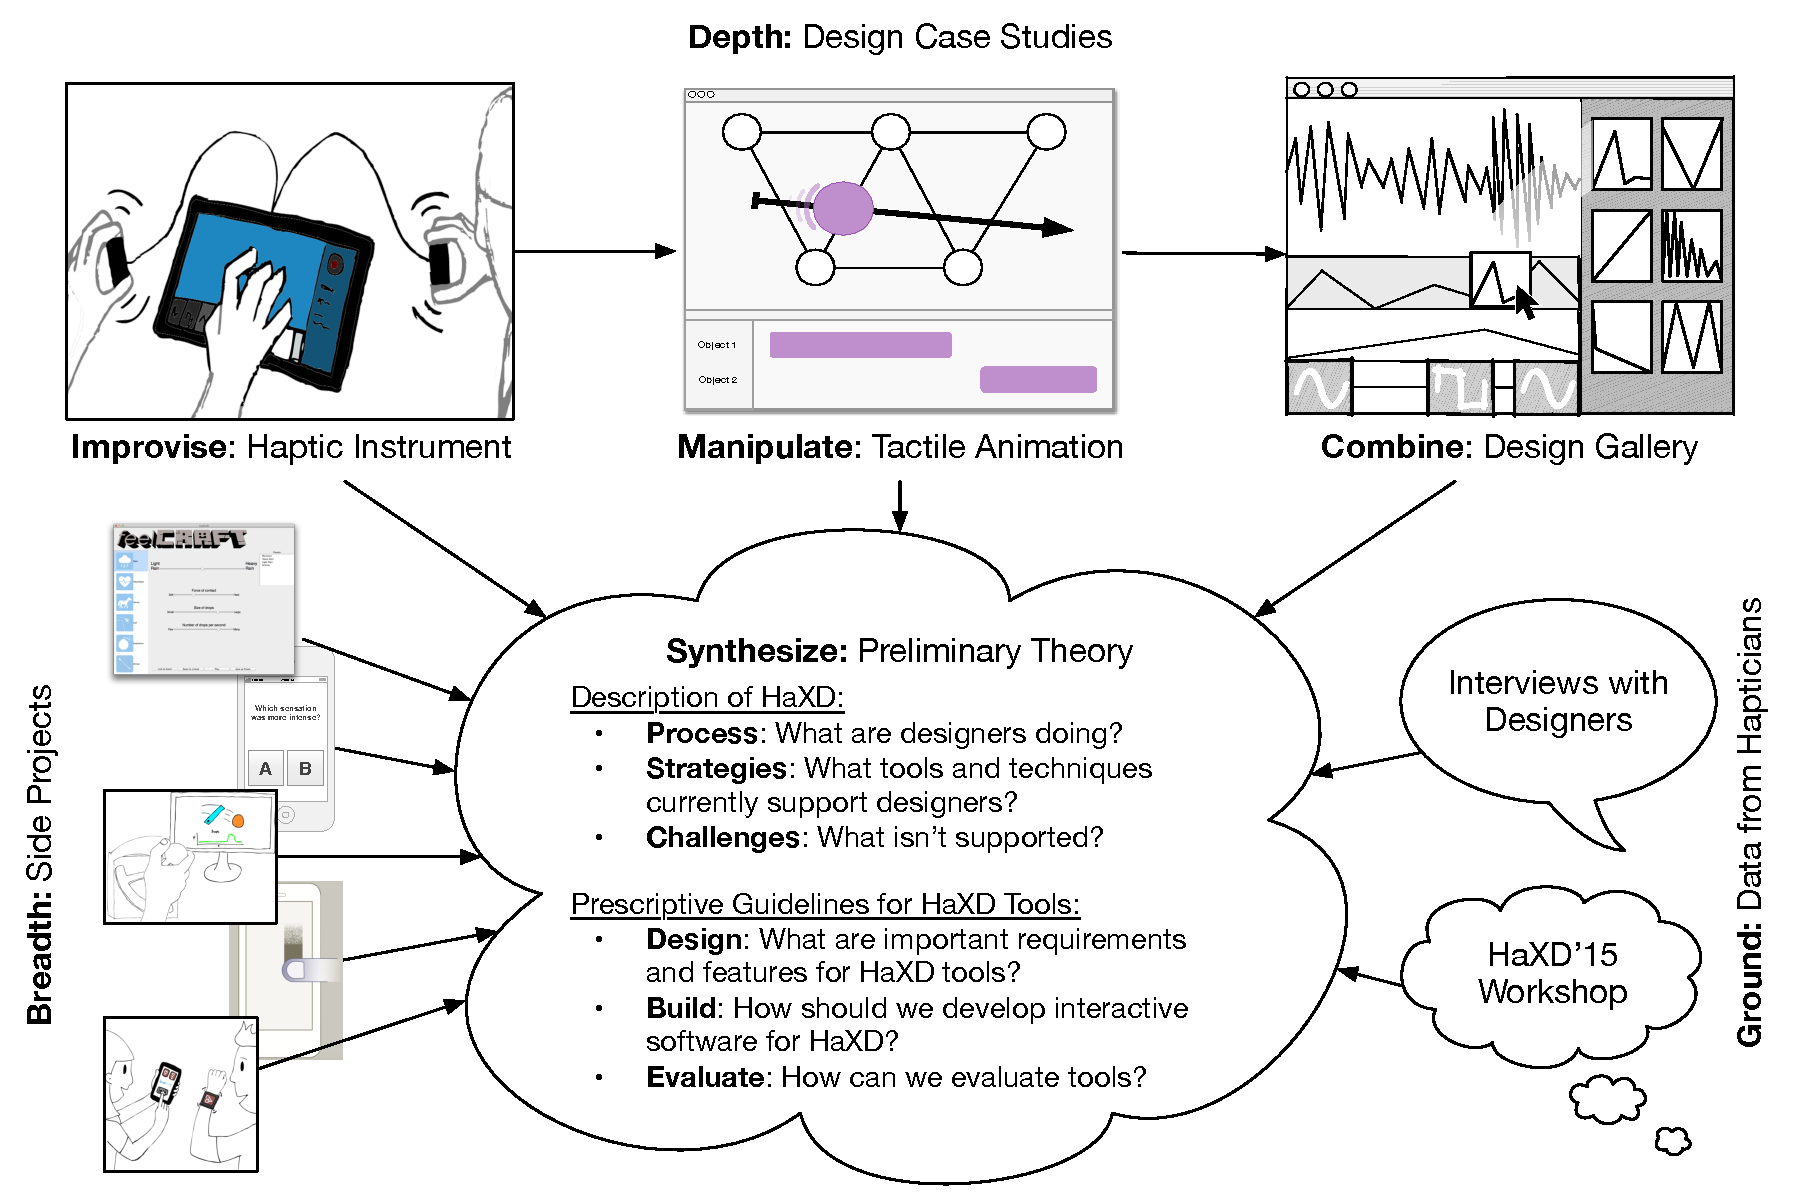
\includegraphics[width=0.7\textwidth]{HaXDTheoryOutline-2015-05-22} 
   \caption{Planned synthesis of data for a preliminary theory of haptic experience design.}
   \label{fig:haxd:theoryoutline}
\end{figure}


The three case studies provide rich but focused data on how to create vibrotactile (VT) experience design tools.
To complement these studies, I propose to gather information more broadly to generalize the haptic design process to other use cases and ground in haptician experience (\autoref{fig:haxd:theoryoutline}).
%from professional haptic designers.
In this way, my final contributions will draw from several sources: 
1) the three in-depth design studies,
%2) a literature survey of general design theories,
2) insight gathered from several side projects, and
3) two sets of grounded data: interviews with professional designers, and
%4) 
%informal interviews with peers at conferences, and 
a workshop at World Haptics `15.

Here, I describe the data collection process, then illustrate possible applications and forms for these contributions.
However, any resulting theory will be emergent from the data, and can take many forms.
To accomplish this in a principled way, I plan to use \emph{memoing} and \emph{constant comparison} \cite{Corbin2008}, looking for common threads between data and double-checking conclusions as new theoretical developments appear.
%This will be guided with a goal: to characterize haptic experience design, especially any features that are unique to this unique class of technological experiences.
This theory will also draw from a literature review of design theory, summarized in this document's related work section.
%This will provide information about non-haptic design disciplines and general theory of design to help frame our inquiry.




%%%%%%%%%%%%%%%%
%
% Section: Data Collection
%
%%%%%%%%%%%%%%%%
\section{Data Collection}
In this section, I list the different sources I intend to use to collect data for theory design.

\subsection{Vibrotactile design case studies}
Each of the  design case studies previously described investigates a specific user group working on a specific VT device with a specific software tool.
Through my experience of gathering requirements, creating tools (through design and development), and evaluating them, I will have first-hand knowledge of supporting aspects of VT sensation design.
Each also produces a small vignette of haptic design in action, giving us glimpses of the design process.

\subsection{Side projects}
In addition to the three design case studies that form this proposal, several side-projects are planned or underway as collaborative efforts.
In these side-projects, I take an organizational or supervisory role, often as summer projects conducted by undergraduates.

\begin{description}
	\item[FeelCraft and Feel Messenger] are collaborations with Disney Research members Ali Israr and Siyan Zhao, looking at distributing and customizing haptic effects in a consumer setting with low-fidelity rumble motor devices.
	I take a haptic designer role to gain a personal understanding of the process, and a software engineer role to understand relevant architectures. % for distributing haptic media.

	\item[CyberHap] is a collaboration between UBC and Stanford looking at force-feedback devices in education; a large team is involved with undergraduate Gordon Minaker leading development of a teaching interface since February 2015, co-supervised by PI Dr. Karon MacLean and me.
%	I co-supervise Gordon with PI Dr. Karon MacLean in this project looking at force-feedback devices in an education setting.
	
	\item[CuddleBit] is a project inspired by the Haptic Creature and CuddleBot project. A small, breathing and vibrating robot will be designed along with a behaviour prototyping tool in summer 2015.
	I supervise undergraduate Paul Bucci in this project exploring multiple modalities and potential for receiving input through a sensor.

	\item[HapTurk] is a collaboration with PhD candidate Hasti Seifi on different techniques to crowdsource feedback on VT icons. Master's student Salma Kashani and undergraduate Matthew Chun are developing visualizations and low-fidelity VT icons during summer 2015.
%	This project looks at a formal mechanism for doing large-scale feedback, and tackles the problem of cross-device and cross-modal equivalency (can a sensation be rendered in some fidelity on both low- and high-fidelity devices?).

	\item[RoughSketch] is a painting application for the TPad Phone, a variable-friction mobile device, for the World Haptics 2015 Student Innovation Challenge. Undergraduates Brenna Li, Paul Bucci, and Gordon Minaker are all fellow team members. Variable friction is a significant contrast to VT sensations as it is intrinsically connected to input: no sensation can be felt without active movement by the user.
\end{description}



\subsection{Grounded Data}
A corpus of interviews with professional haptic designers has already been collected by UBC alumni Colin Swindells during his PhD, but has never been published.
I will analyze these interviews to further ground our findings with real-world haptic designers.

To complement this %, and because professional haptic designers are rare and difficult to find,
we turn to the research community who do design as part of their work.
The planned Workshop on Haptic Experience Design (http://oliverschneider.ca/HaXD) at World Haptics 2015 will also provide a data source.
At this workshop, 4 experts of haptic experience design will speak, participants will reveal their own design challenges in a brainstorming activity, and the ensuing panel discussion should help illuminate practices and paths for future work.

%%%%%%%%%%%%%%%%
%
% Section: Possible Format
%
%%%%%%%%%%%%%%%%
\section{Possible Format}
While the theory can take many forms, I hope to characterize haptic experience design and contrast it with other design fields, especially graphic and audio design.
I hope to find both descriptive and prescriptive results, including current practices, an identification of challenges uniquely facing haptic designers, and guidelines for designers and developers of haptic design support tools.

\subsection{Descriptive Contributions: HaXD Process as Requirements}
My first goal is to describe the \textbf{processes} employed by haptic designers.
This could manifest, for example, as a catalogue of 
existing haptic design tools,
appropriated tools (e.g., using a sound editor to create VT icons),
techniques (e.g., design philosophies like Haptic Sketching),
resources (e.g., libraries and APIs),
platforms (what devices designers are using),
practices in haptics education (undergraduate or graduate level courses),
and tasks undertaken by haptic designers.

For example, to share of haptic experiences, haptic designers create demos
to spread awareness of haptic research and gain feedback from peers.
%One colleague, upon being introduced to the Haptics Symposium conference, said that the haptics community gets demos right.
This is so ingrained into the culture of haptic research that recently a demo-only conference was launched: Asia Haptics.

Once collecting a description of current practices, I expect we might be able to identify \textbf{challenges} and \textbf{strategies} to addressing those strategies, including the ecosystem of available tools: what is working well, and what is broken.
Using our example of collaboration and demos, we might see that in-person demos are effective, but
remote collaboration or asynchronous sharing is challenging. %, but could offer more frequent collaboration between designers.
Available tools include videos and visualizations of demos to explain concepts in lieu of the demo itself.
%Other challenges might include the great variety of different devices, non-haptic tools appropriated for haptic design, the implementation complexity of dealing with hardware, low-level software, and application logic simultaneously, or the strong influence of other modalities (vision, hearing) on perceived touch sensations.

\subsection{Prescriptive Contributions: Guidelines for HaXD Software Tools}
After describing HaXD as a set of requirements, I will then develop guidelines for how to built supportive interactive software tools.
Right now, I plan to organize this into three aspects: how to \textbf{design} tools, including important features relevant to different stages of HaXD; how to \textbf{build} tools, including relevant software architectures and ways to address technical challenges; and how to \textbf{evaluate} tools, methods to capture designer experience and inform future design.

Hypothetical use cases might best explain this contribution.
One examples is using these guidelines for knowledge transfer to industry.
I could use these guidelines to advise or create design software for companies developing haptic hardware platforms (such as the TPad team and UltraHaptics) or software platforms (such as Immersion and Phidgets), bridging the gap from research to industry application.
Another example could be dissemination through haptics education.
Developing a module for a haptic design course, such as CPSC 543, is an accessible way to encapsulate and test these ideas.
This could also manifest in a multi-day workshop, similar to Camille Moussette's Haptic Sketching workshops, to validate ideas at different institutions.



\section{Deliverables and Risk}
There are two expected deliverables from this theory development.
First, the HaXD'15 workshop on Haptic Experience design is planned, piloted, and scheduled for World Haptics in June, 2015. 
To get the most out of this workshop, photographs and notes will be recorded.
Afterwards, a very small digest piece debriefing the workshop is planned in winter 2016; this may be submitted on its own as an short paper if an appropriate venue is available (e.g., a special journal issue similar to \cite{Jones2014}), or subsumed into the second deliverable.

The second deliverable is a retrospective piece on our findings from all the data sources found here, but with a focus on data from haptic designer interviews.
This interview data has already been collected by UBC alumnus Colin Swindells.
I plan to digest and analyze those interviews in winter 2016 to generate requirements grounded in designer experience.
This will likely be combined with synthesized findings from the three design studies and several side projects.
To mitigate risk, we can combine interview findings to a greater or lesser extent with other data sources.
If the interviews have a great deal of information, they could be a valuable contribution on their own.
If not, I expect them to supplement our other data sources.
This document will likely be submitted as a full paper to a peer-reviewed conference or journal.

Within each project, we mitigate risk through strategic planning and study design;
many of these projects do not have to be successful to provide input.
For example, HapTurk may never actually be deployed, but could still articulate the challenge of a large-scale, remote haptic user study.
In addition,
risk is partially managed through sheer attrition: one or two side projects or data sources could provide limited feedback and we would still have a diverse set of information. 
However, I will note that initial investigation has already been useful.

%
%To ground our other findings with our target end users, and identify challenges that may not emerge from the literature alone.
%The goal is to develop an initial proposed theory of haptic experience design from multiple sources, which characterizes the unique process that can or could support designers.
%I plan to gather information from a variety of sources, including interviews with professional designers, informal interviews with peers during conferences, and the literature.


%The main source of data will be from interviews with professional designers, several of which have been collected already by researcher Colin Swindells.
%These will be analyzed using qualitative techniques like grounded theory and phenomenology \cite{Creswell2013, Moustakas1994}.
%
%A second source of data will be reflection on our own projects and those of our peers and collaborators.
%
%
%Currently, much of the literature review has already been conducted for this document, 
%





%% KM - for comments
%\newcommand{\inlinecomment}[3][]{$\lceil$\textbf{#1}~\textit{\textcolor{#2}{#3}}$\rfloor$}
%\definecolor{DarkGreen}{rgb}{0.0, 0.5, 0.0}
%\definecolor{DarkRed}{rgb}{0.7, 0.2, 0.2}
%\definecolor{DarkOrange}{rgb}{1, 0.5, 0}
%\definecolor{Orange}{rgb}{1, 0.75, 0}
%\newcommand{\kmC}[1]{\noindent \inlinecomment[KM]{DarkGreen}{#1}}
%\newcommand{\kmE}[1]{\textcolor{DarkRed}{#1}}
%\newcommand{\osC}[1]{\noindent \inlinecomment[OS]{Orange}{#1}}
%%\newcommand{\osC}[1]{}
%\newcommand{\osE}[1]{\textcolor{DarkOrange}{#1}}
%
%%Organization commands
%\newcommand{\inlineHeading}[1]{\emph{#1} --}
%
%%\newcounter{pathwayCounter}
%\newcommand{\challenge}[1]{\textbf{Pathway: #1} --}
%
%
%Although haptic technologies have become commonplace in end-user experiences, there are still few established processes to guide designers, who face special challenges that arise out of the relative youth of the field and from qualities intrinsic to the sense of touch.
%Design guidelines, toolkits, and authoring interfaces exist as disparate pieces of knowledge rather than a unified perspective, 
%hobbling the creativity and efficiency needed to create new haptic experiences. 
%In this paper, we assemble key elements of the haptic design process and its
%needs
%into a generalized
% framework and vocabulary, 
%to promote
% a more fluid, extendable, and transferrable understanding of the practice, 
%guide development of effective tools, and 
%promote a discourse around both. 
%We begin with haptic versions of three primary
% design activities identified in
% design theory, creativity support tools, and other fields of design: problem preparation, hands-on design, and collaboration.
%These activities form a framework by which we can organize the haptic design literature and our own experience 
%into specifically defined
%pathways for design, identifying areas for future research and implications for tool development.
%
%
%
%
%\begin{table*}
%\caption{Design Activities, Sub-Activities, and Pathways Synthesized from the Literature}
%\label{tab:designactivities}
%
%%
%%
%%% Old version - horizontally laid out
%%
%%\begin{center}
%%	\begin{tabular}{|c|c|c|c|c|c|c|c|c|}
%%	\hline
%%		
%%		
%%	\multicolumn{3}{|c|}{\bf Problem Preparation (\Cref{sec:problempreparation}) }
%%		& \multicolumn{3}{|c|}{\bf Hands-on-Design (\Cref{sec:handsondesign})}
%%		& \multicolumn{3}{|c|}{\bf Collaboration (\Cref{sec:collaboration})} \\
%%		
%%		\multicolumn{3}{|c|}{\emph{Use the Designer's Experience}}
%%		& \multicolumn{3}{|c|}{\emph{Navigate a Design Space}}
%%		& \multicolumn{3}{|c|}{\emph{Design together}} \\
%%		
%%	\hline
%%		
%%	Framing
%%		& Repertoire
%%		& Examples
%%	& Ideation
%%		& Evaluation
%%		& Sketching
%%	& Relate
%%		& Feedback
%%		& Donate \\
%%		
%%	%sub-activities
%%	\emph{Defining}
%%		& \emph{Internal}
%%		& \emph{External}
%%	& \emph{Generation}
%%		& \emph{Filtering}
%%		& \emph{Rapid, flexible,}
%%	& \emph{Informal talks}
%%		& \emph{Formal studies}
%%		& \emph{Dissemination} \\
%%		
%%	\emph{the problem}
%%		& \emph{experience}
%%		& \emph{resources}
%%	& \emph{of ideas}
%%		& \emph{of ideas}
%%		& \emph{ambiguous notation}
%%	& \emph{with peers, mentors}
%%		& \emph{with users}
%%		& \emph{to community} \\
%%		
%%%	\hline	
%%%	%Challenges
%%%	\emph{Flexible interfaces,}
%%%		& \emph{Accessible}
%%%		& \emph{Example}
%%%	& \multicolumn{2}{|c|}{Support multiple}
%%%		& \emph{Support ambiguity,}
%%%	& \multicolumn{3}{|c|}{Challenge: \emph{investigate asynchronous,}} \\
%%%		
%%%	\emph{multiple views}
%%%		& \emph{knowledge}
%%%		& \emph{management}
%%%	& \multicolumn{2}{|c|}{parallel designs}
%%%		& \emph{commenting, abstraction}
%%%	& \multicolumn{3}{|c|}{ \emph{distributed collaboration}} \\	
%%		
%%	\hline
%%	\end{tabular}
%%\end{center}
%%\end{table*}
%%
%
%
%\begin{center}
%	\begin{tabular}{lll}
%	\toprule
%		
%
%%	\rowcolor [gray]{.8}
%	\textbf{Activity}
%		& \textbf{Sub-Activity}
%		& \textbf{Pathways for Design}
%		\\
%	\midrule
%	
%	\multirow{3}{1.7in}{\textbf{Problem Preparation (\Cref{sec:problempreparation})} \emph {Use the Designer's Experience}}
%		& Framing -- Defining the problem
%		& Flexible interfaces, multiple views, powerful language
%		\\
%	\cmidrule{2-3}
%		& Repertoire -- Internal experience
%		& Task-based knowledge source
%		\\
%	\cmidrule{2-3}
%		& Examples -- External resources
%		& Manage examples: capture, find, access, transform
%		\\
%	\midrule
%	
%	\multirow{3}{1.7in}{\textbf{Hands-on Design (\Cref{sec:handsondesign})} \emph {Navigate a Design Space}}
%		& Ideation -- Generate ideas
%		& \multirow{2}{*}{Explore multiple design candidates in parallel}
%		\\
%	\cmidrule{2-2}
%		& Evaluation -- Filter ideas
%		&
%		\\
%	\cmidrule{2-3}
%		& Sketching -- Rapid, flexible, ambiguous notation
%		& Support speed, ambiguity, commenting, abstraction
%		\\
%	\midrule
%	
%	
%	\multirow{3}{1.5in}{\textbf{Collaboration (\Cref{sec:collaboration})} \emph {Design Together}}
%		& Relate -- Informal talks with peers, mentors
%		& \multirow{3}{*}{Explore asynchronous and distributed interactions}
%		\\
%	\cmidrule{2-2}
%		& Feedback -- Formal studies with users
%		&
%		\\
%	\cmidrule{2-2}
%		& Donate -- Dissemination to community
%		&
%		\\
%	
%		
%%	\multicolumn{3}{|c|}) }
%%		& \multicolumn{3}{|c|}{\bf Hands-on-Design (\Cref{sec:handsondesign})}
%%		& \multicolumn{3}{|c|}{\bf Collaboration (\Cref{sec:collaboration})} \\
%%		
%%		\multicolumn{3}{|c|}{\emph{Use the Designer's Experience}}
%%		& \multicolumn{3}{|c|}{\emph{Navigate a Design Space}}
%%		& \multicolumn{3}{|c|}{\emph{Design together}} \\
%%		
%%	\hline
%%		
%%	Framing
%%		& Repertoire
%%		& Examples
%%	& Ideation
%%		& Evaluation
%%		& Sketching
%%	& Relate
%%		& Feedback
%%		& Donate \\
%%		
%%	%sub-activities
%%	\emph{Defining}
%%		& \emph{Internal}
%%		& \emph{External}
%%	& \emph{Generation}
%%		& \emph{Filtering}
%%		& \emph{Rapid, flexible,}
%%	& \emph{Informal talks}
%%		& \emph{Formal studies}
%%		& \emph{Dissemination} \\
%%		
%%	\emph{the problem}
%%		& \emph{experience}
%%		& \emph{resources}
%%	& \emph{of ideas}
%%		& \emph{of ideas}
%%		& \emph{ambiguous notation}
%%	& \emph{with peers, mentors}
%%		& \emph{with users}
%%		& \emph{to community} \\
%		
%%	\hline	
%%	%Challenges
%%	\emph{Flexible interfaces,}
%%		& \emph{Accessible}
%%		& \emph{Example}
%%	& \multicolumn{2}{|c|}{Support multiple}
%%		& \emph{Support ambiguity,}
%%	& \multicolumn{3}{|c|}{Challenge: \emph{investigate asynchronous,}} \\
%%		
%%	\emph{multiple views}
%%		& \emph{knowledge}
%%		& \emph{management}
%%	& \multicolumn{2}{|c|}{parallel designs}
%%		& \emph{commenting, abstraction}
%%	& \multicolumn{3}{|c|}{ \emph{distributed collaboration}} \\	
%		
%	\bottomrule
%	\end{tabular}
%\end{center}
%\end{table*}
%
%
%
%
%%%%%%%%%%%%%%%%%%%%%%%%%%%%%%%%%%%%%%%%%%%%%%%%%%%%%%%%%%%%%%%%%%%%%%%%%%%%%%%%%
%\section{Introduction}
%Haptic technology has become a 
%standard ingredient of user interactions with technology, with the potential to add engagement to media experiences \cite{Modhrain2001, Danieau2014} and ``calm'' everyday interactions \cite{MacLean2009}.
%% No longer restricted to research labs or theme park rides, 
%Carefully designed and expressive haptic feedback is finding its way into commercial devices, most recently the Apple Watch (www.apple.com/watch).
%
%
%
%\begin{figure}[tbp] %  figure placement: here, top, bottom, or page
%	\centering
%	\begin{subfigure}[b]{0.23\textwidth}
%		   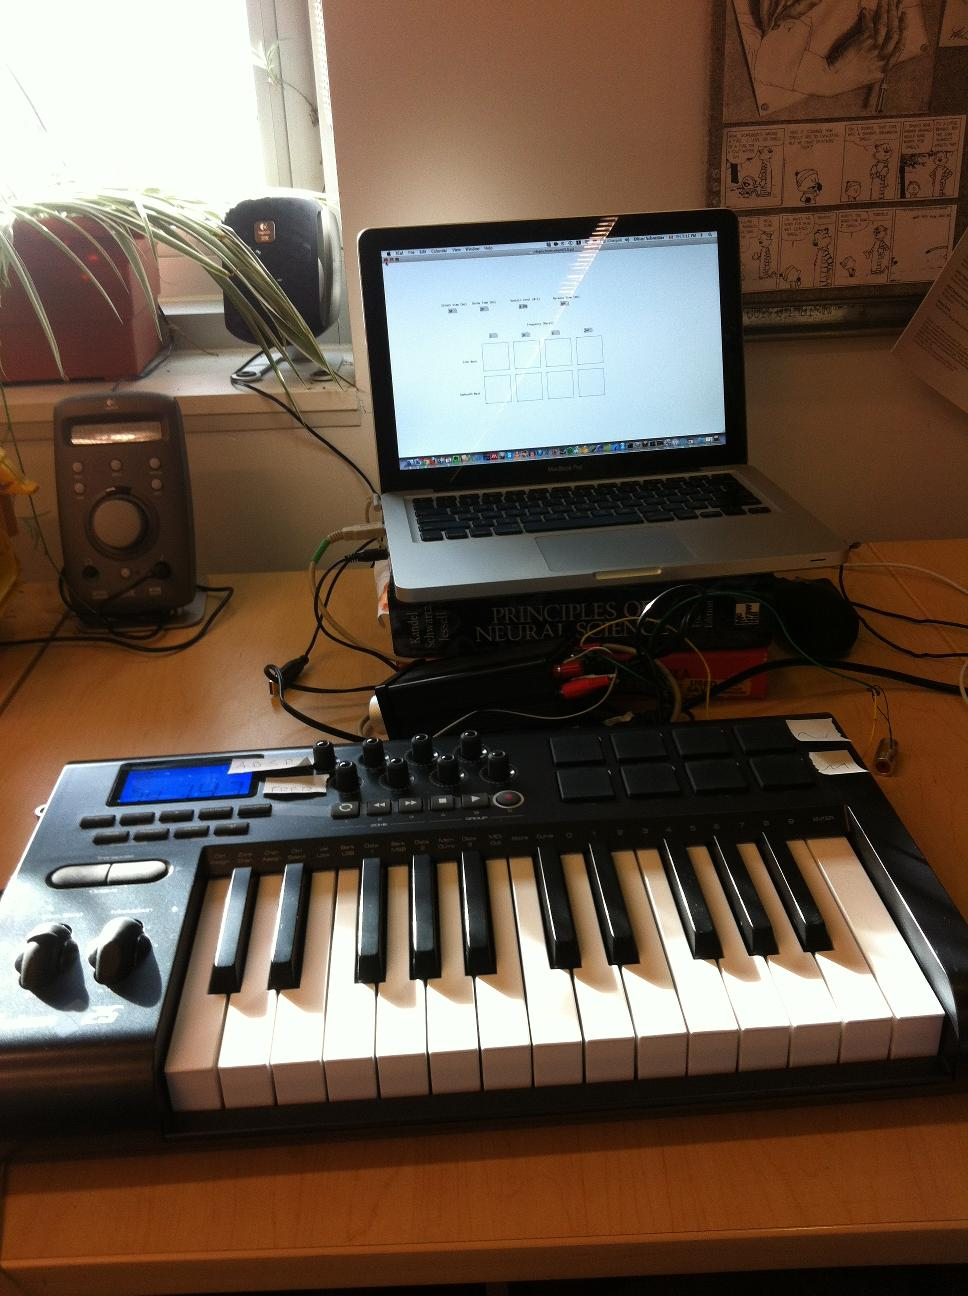
\includegraphics[height=2.3in]{figures/HIVE-photo} 
%		   \caption{Early hardware sketch}
%		   \label{fig:example:hardware}
%	\end{subfigure}
%	\quad
%	\begin{subfigure}[b]{0.22\textwidth}
%		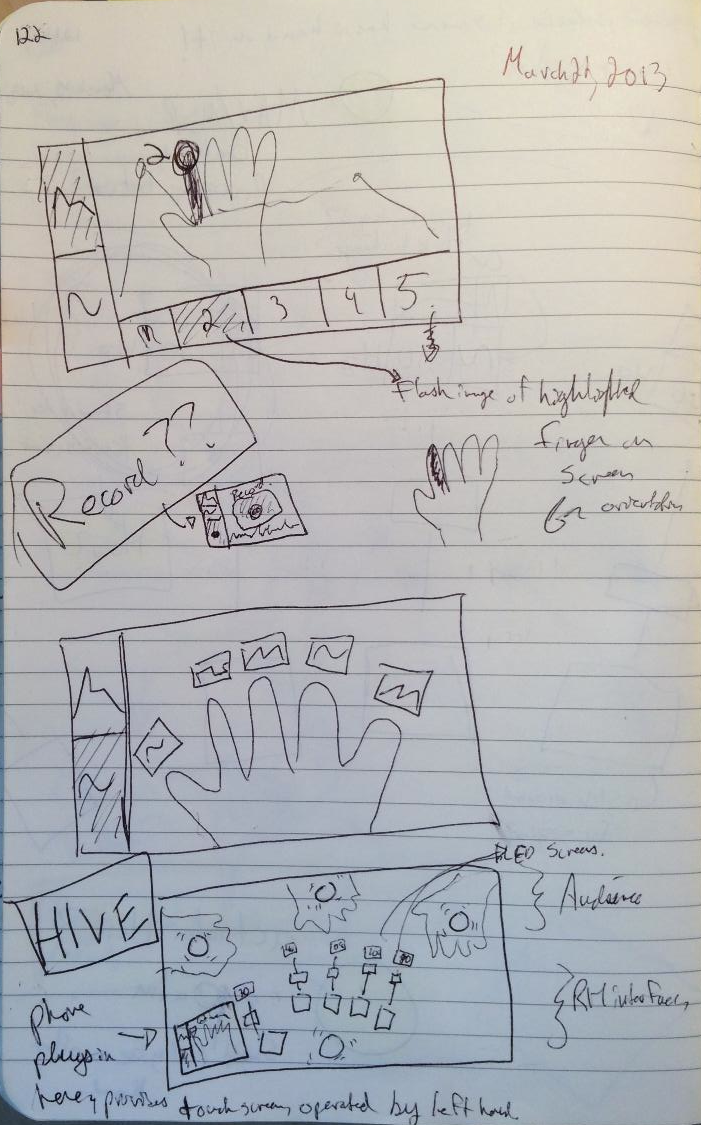
\includegraphics[height=2.3in]{figures/mHIVE-earlysketch-photo-cropped} 
%		\caption{Early paper sketch}
%		\label{fig:example:paper}
%	\end{subfigure}
%	\caption{Early sketches for mHIVE \cite{Schneider2014} in hardware (a) and on paper (b), showing a \emph{framed} approach (instrument metaphor), inspiration from the designer's \emph{repertoire} (musical experience), and extension of \emph{examples} (dials and buttons adapted from the keyboard).}
%	 \label{fig:example}
%\end{figure}
%
%
%% Despite this growth, 
%Nevertheless, there is no established process for haptic experience design (``HaXD").
%% (HaXD) %OS: We never reuse this, but may want to in future drafts
%% has no established design process.
%% One culprit is the small and fragmented user base:
%Culprits abound. The user base is small and fragmented:
%professional haptic designers are still rare, often share engineering or scientific duties, and tend to be sequestered in companies whose business needs preclude broader interactions % with other designers.
%and complicate observation of design practices by researchers.
%%\kmE{They lack both training in an articulated user-experience design approach, and an interlinked community through which they can consolidate vocabulary and share best practices.}
%It is difficult to translate guidelines from other fields, in absence of analogies to % graphic design's 
%colour % theory 
%or musical theory. % for touch.
%Designing for the sense of touch entails % brings intrinsic design challenges, such as  %as it involves 
%hard-to-prototype hardware and context-sensitive perception~\cite{Hayward2008}.
%
%%However, when attempting to get that ineffable quality of getting something to ``feel right" in a given context, a robust design process can help when prescriptive guidelines fail.
%
%Recently, design thinking applied to haptics \cite{Moussette2012} has added to the literature on HaXD process \cite{Swindells2006}.
%Toolkits \cite{Minamizawa2012,Ledo2012}, effect libraries \cite{Israr2014},  collaborative software \cite{Ruthenbeck2014,Cha2009} and interfaces themselves \cite{Schneider2014} ease production of haptic \emph{effects}.
%However, a systematic, convergent procedure by which haptic \textit{experiences} can be developed
%to meet specific requirements -- which themselves may be hard to articulate -- is elusive, % not well defined, 
%with previous work providing only % isolated elements. % 
%pieces of the puzzle.
%
%In this paper, we aim to situate
%haptic design tasks in a common framework.
%Synthesizing insights from design and creativity literature, we describe
% three critical activities conducted during many types of design: 
% \textit{problem preparation}, \textit{hands-on design}, and \textit{collaboration}, each with
% sub-activities.
%We discuss each in the haptic context to discover what activities are supported and which are not,
%with examples drawn from literature and our personal experience as designers and observers of other designers.
%This design lens
%reveals not only a process, but pathways for more focused investigation, informing the creation of HaXD support tools.
%
%
%
%%\inlineHeading{Design Activities}
%
%
%%\begin{table}
%%\caption{Problem Preparation Sub-Activities}
%%\label{tab:problem:preparation}
%%\begin{center}
%%	\begin{tabular}{|l|p{2cm}|p{2cm}|p{2cm}|}
%%	\hline
%%		&Description	&Haptics so far	& Haptics next	\\
%%	
%%	
%%%	\hline
%%%	\textbf{Problem Preparation}	&	&	&	\\
%%	
%%		\hline
%%		\emph{Framing}
%%			& transforming the problem into a manageable form
%%			& Ongoing investigation of haptic language, perceptual dimensions
%%			& Flexible, adaptable tools; multiple views	\\
%%
%%		\hline
%%		\emph{Repertoire}
%%			& building the designer's internal experience
%%			& Haptics education (e.g., HapKit,  Twiddler), DIY haptics, haptic illusions
%%			& Handbook, wiki, or other more elaborate compendium of knowledge	\\
%%		\hline
%%		\emph{Examples}
%%			& Drawing from external resources and designs
%%			& Haptic camera, libraries (Immersion, Upenn, FeelEffects), haptic search engine
%%			& Capture \& upload, find (search/explore/visualize), use (design galleries, editable data types)	\\
%%	\hline
%%	\end{tabular}
%%\end{center}
%%\end{table}
%
%
%
%%\subsection{Challenge: Difficult Problem Framing}
%%The CHALLENGES (unfilled holes):
%%
%%1. Problem Gathering:
%%No Language, limited theory (framing)
%%Complex sense (hard to understand, need to be expert in multiple domains
%%) (repertoire+framing)
%%No language/theory
%%limited ways to capture, render, maintain examples
%
%
%\challenge{Multiple metaphors}
%Despite a steady progression of research on perception,
%there is no agreed upon language for working with haptics \cite{Obrist2013,Okamoto2013,Jansson-Boyd2011}.
%Most authoring tools have relied on fixed metaphors and devices, limiting \emph{framing}.
%Allowing  multiple metaphors or views on a haptic design is one way in which a designer can % would allow the designer to 
%reshape a problem to be easier to solve (reframe it so it matches their \emph{repertoire} or found \emph{examples}).
%Future authoring tools should pursue flexibility or improved abstractness.
%%Abstract metaphors could apply to multiple device classes, .
%
%%Examples:
%%?	Haptic Camera
%%?	Kuchenbecker?s haptic textures
%%?	Libraries
%%?	Feel Effects/FeelCraft
%%?	Ultrasound Examples from Keisuke Hasegawa?s HaptoMime at AsiaHaptics:
%%o	Tried a bunch of waveforms extracted from sound sources in the Komplete audio packagewith my own palm. It?s a pity that there was no systematic procedure to determine what waveform to pick up. My only advice is that it would be good and efficient to construct an experimental system which allows you to test many kinds of stimuli promptly at an early stage in y our researches.
%%?	Need examples from industry
%
%
%
%%\kmC{Isn't this a library not an education problem? SLC} % Not following the focus on haptics education here, as related to repertoire. Can you strengthen the connection? I thought this particular challenge would be more about how designers can capture, organize, find, reuse externally sourced inspiration and examples - essentially, the library problem. Education, and communication with one another, is an important but different challenge.}
%% That said, I am still fuzzy on distinction between repertoire and examples. They both need libraries, don't they? Because there are a lot of them, and the point is re-use. 
%\challenge{Task-based knowledge}
%To build their \emph{repertoire}, haptic designers must learn essential haptics concepts and begin solving relevant problems.
%Haptics courses \cite{Okamura2012, Jones2014} often provide a HaXD practitioner with initial experience.
%Brief, cogent outlines  of haptics knowledge (e.g., \cite{Hayward2007,MacLean2008,Hayward2008,Karam2013}) allow designers to expand their experience in an accessible way, and resources like EduHaptics (eduhaptics.org) link designers to content.
%However, knowledge is still framed with disparate perspectives. 
%The next step is to understand the low-level tasks conducted in HaXD.
%This would enable development of a more focused ``how-to" compendium of knowledge uniting perception, hardware, and software knowledge bases.
%%Ideally, this will link directly to HaXD tasks, but more research is needed to understand the .
%%, but still accessible, source of knowledge; a handbook of haptics knowledge that summarizes perceptual research, lists prominent examples of design, and guidelines for design and development.
%%This need not be a traditional handbook, but could be an online tool, such as a wiki or online course.
%%A proposed handbook might have more content internalized, structured to be handy and self contained, featuring design case studies.
%
%%\emph{Examples}
%\challenge{Manage examples}
%Currently, \emph{examples} exist in several libraries (e.g., \cite{Culbertson2014, Israr2014}), but capturing, organizing, accessing, and transforming them poses a greater challenge for haptic design than for more visually oriented, or even auditory, domains.
%%Excluding progress made by expanding these libraries in scale or in device support, there are key areas we can look for future progress.
%Capturing with a haptic camera  \cite{MacLean1996} is useful, but limited to that camera's target phenomenon.
%Integration of library uploads into authoring tools (e.g., as suggested in \cite{SchneiderAsiaHaptics2014}), would make it easier to grow a set of \emph{examples}.
%Visualizations, searching techniques (like a haptic search engine \cite{Adi2010,Hanamitsu2014}), and browsing techniques will facilitate access.
%%One demoer at a recent conference described his approach to create a tactile effect.
%%He tried waveforms extracted from sound sources in the Komplete audio package, stating ``It's a pity that there was no systematic procedure to determine what waveform to pick up" and wishing for a system to try stimuli at an early stage.
%%with my own palm. It?s a pity that there was no systematic procedure to determine what waveform to pick up. My only advice is that it would be good and efficient to construct an experimental system which allows you to test many kinds of stimuli promptly at an early stage in y our researches.
%%In haptics, we have already done some work on capturing examples, for example, the haptic camera \cite{MacLean1996}, or empirically gather libraries \cite{Culbertson2014}.
%% Some examples or templates are often shipped with toolkits (Verify!), and recently vibrotactile libraries have been developed: Immersion, Feel Effects, or the UPenn surface toolkit \cite{Culbertson2014}.
%%The haptic search engine (asia haptics) is one way of recalling examples.
%Finally, current \emph{examples} are static -- the designer chooses one and adds it to their application.
%%Novel techniques of using examples to create new designs.
%Open, manipulatable formats beyond parameters (like those in \cite{Ledo2012,Israr2014}) or through design galleries \cite{Lee2010a,Marks1997} is an exciting avenue to allow designers to work hands-on with \emph{examples}.
%
%%Originating in the graphics literature, design galleries provide a set of designs similar or different from your current design, letting users take interesting parameters and apply them to their design \cite{Marks1997}.
%%This idea has since been applied to other design fields like web design \cite{Lee2010a}.
%%Given the difficulty of framing with no fixed haptic parameters or language \cite{Jansson-Boyd2011}, example-based design could be a promising avenue for future design tools.
%%It's also been recommended that focusing on rapid prototyping can get around language barriers in haptics \cite{Fogg1998}.
%%To do this, we need to focus on hands-on design of haptics, the second major design activity.
%
%
%
%%Rapid iteration is essential for being able to think by doing; creativity support tools must have a low threshold, high ceiling, and wide walls: accessible to beginners, powerful for complete solutions, and support a wide range of explorations \cite{Resnick2008}.
%%A sketch can have many purposes, but is distinguished from a prototype by being more generative, less complete, and characteristic of earlier design \cite{Buxton2007}.
%
%
%
%
%%Donald Sch\"{o}n's seminal book, The Reactive Practitioner, describes the process of
%%learning skills to be one of reflection-in-action. That is, a pitcher in a baseball game must be able to find their groove. Through a process of subtle adjustment and experimentation, a pitcher adjusts her technique to fit the current, myriad conditions the wind, the current batter, the sun; the list goes on. This process is implicit, and often people find it impossible to articulate. Like the poor centipede, we sometimes find it difficult to realize that knowledge is embedded in our action, and in fact it can ruin our stride. Verbal overshadowing, articulating a wine's taste or a person's face, often weakens our memory unless we've been trained to verbalize those notions \cite{Schooler1990}. Similarly, a haptic designer must adapt to her design project to the current conditions.
%
%%Idea generation vs Idea evaluation. Sketching.
%
%
%%\begin{figure}[htbp] %  figure placement: here, top, bottom, or page
%%   \centering
%%   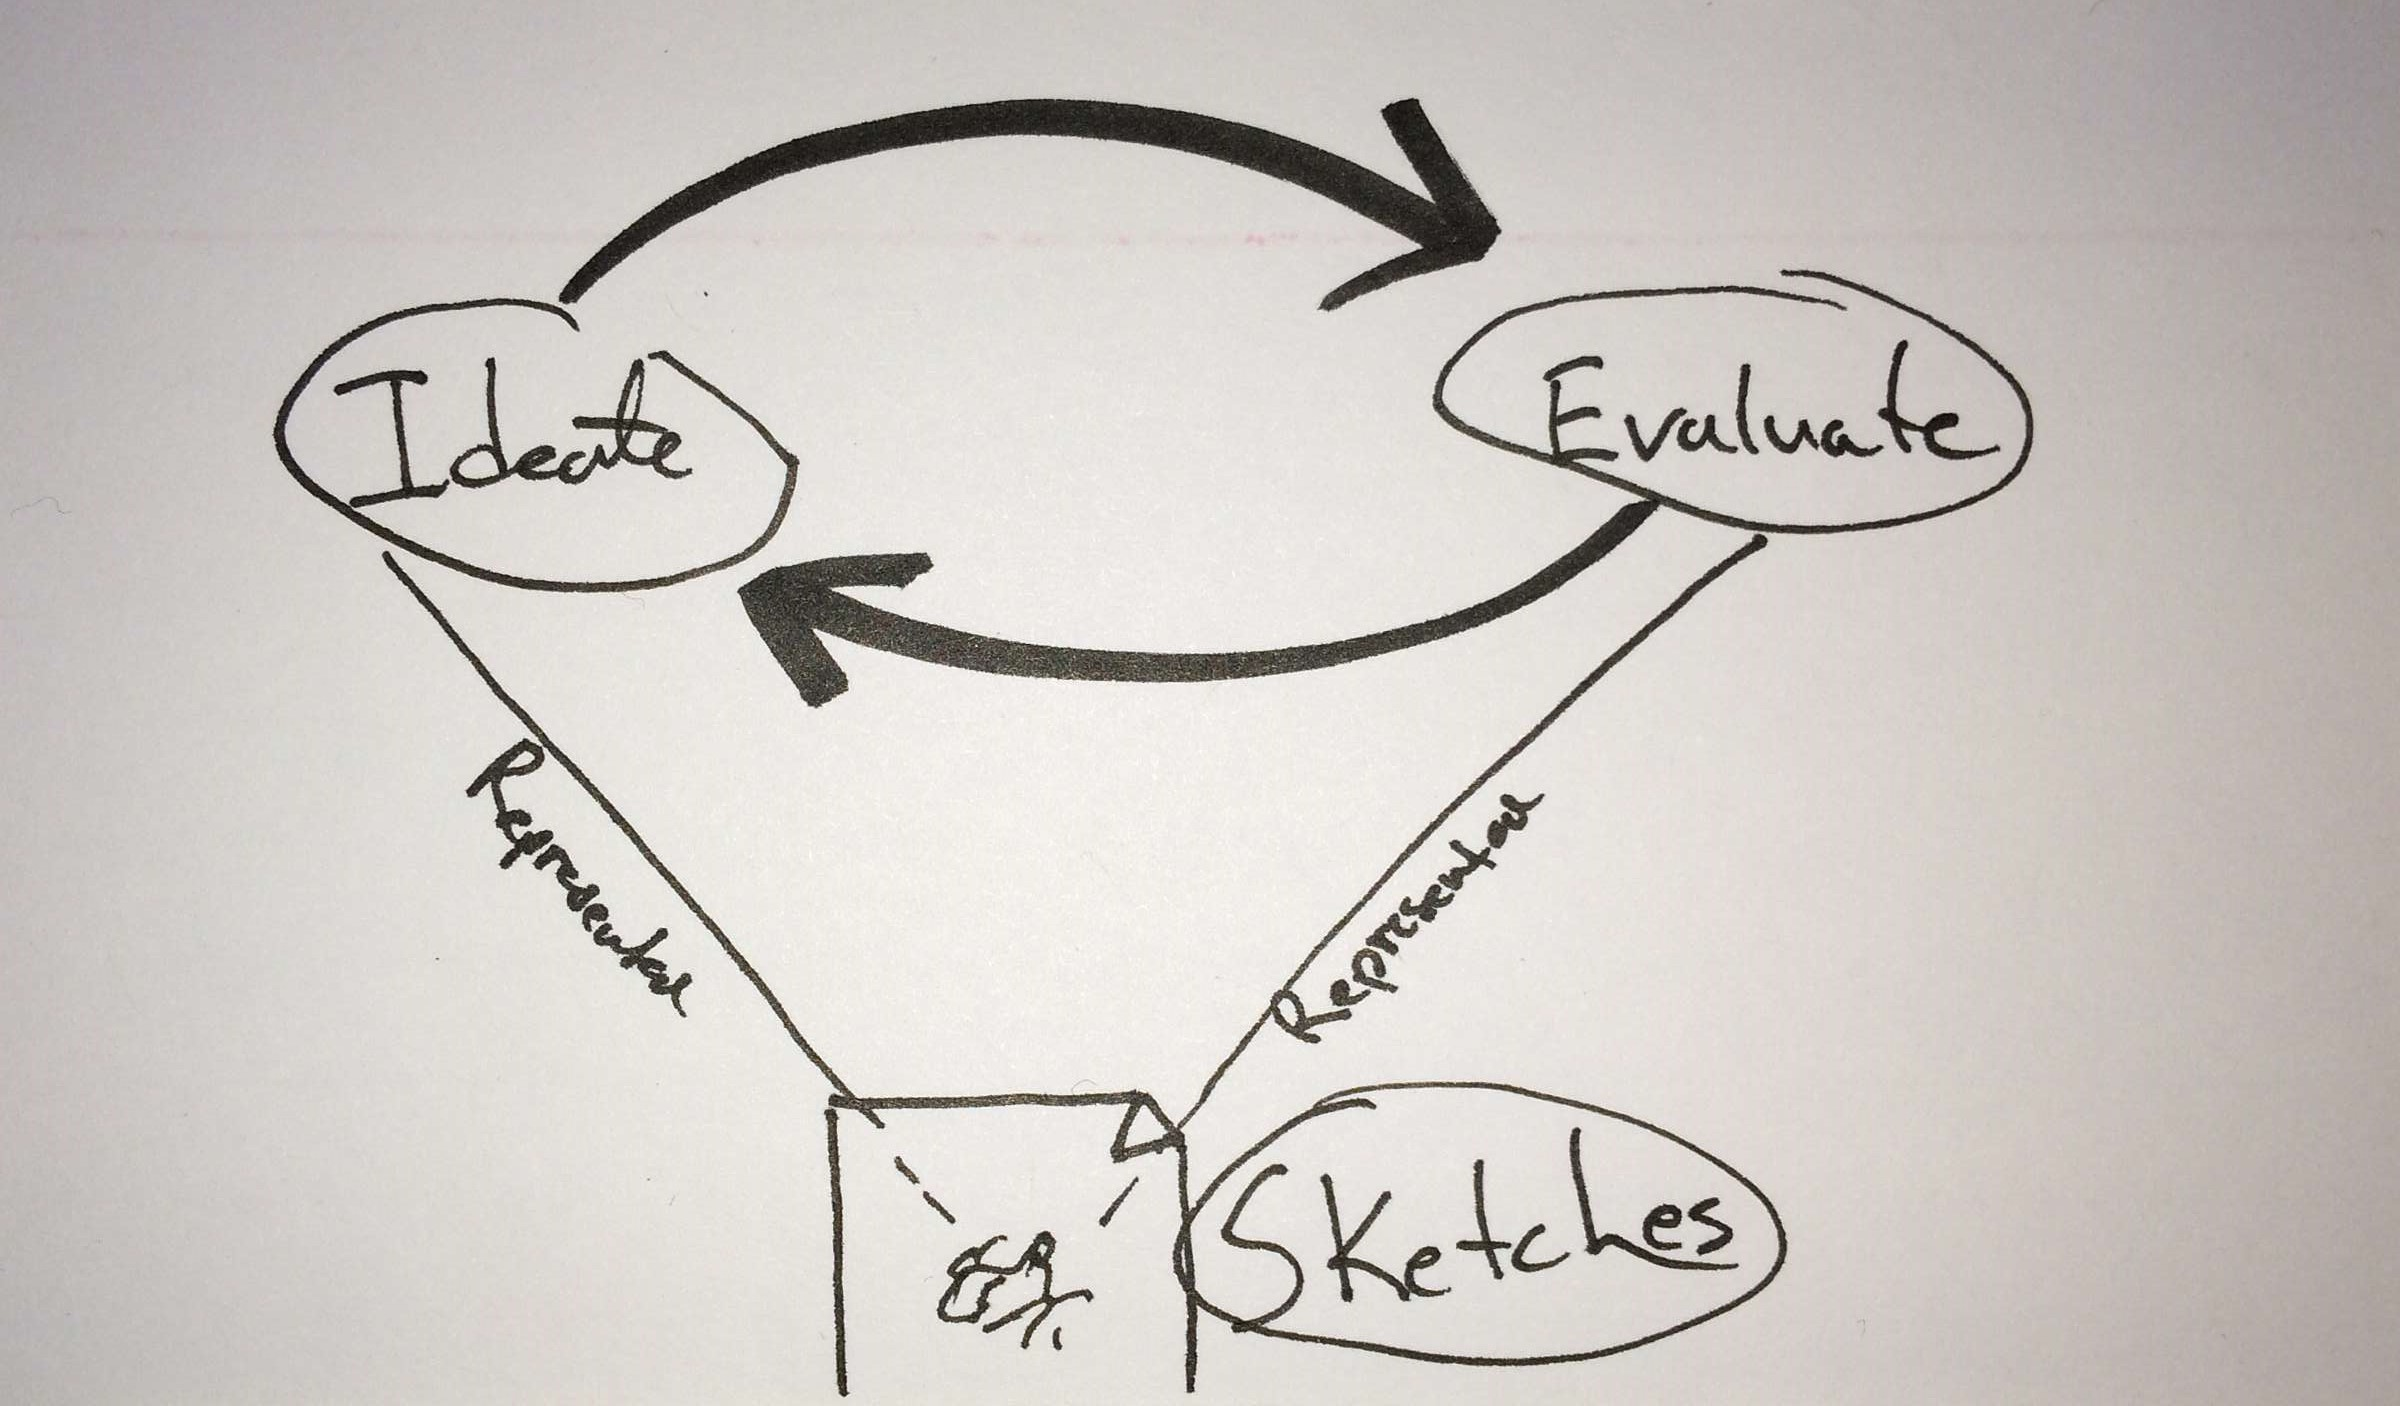
\includegraphics[width=0.48\textwidth]{figures/HandsOnDesignSubProcessesPlaceHolder} 
%%   \caption{Hands-on design sub-activities. Designers iterate between ideation and evaluation, representing this process through sketches.\textbf{(PLACEHOLDER)}}
%%   \label{fig:hands:on:sub:activities}
%%\end{figure}
%
%
%\challenge{Multiple, parallel designs}
%Ideation and evaluation are partially supported by existing tools.
%Parallel development of interfaces has been applied to physical UIs with Arduino \cite{Hartmann2008}.
%Brainstorming and techniques like A/B testing, comparing two designs side-by-side, have been employed in haptics design tools \cite{Swindells2014}.
%Rapid ideation and evaluation are also supported through better framing tools like design galleries, described in the previous section.
%
%\challenge{Ambiguity, commenting, \& ad-hoc use}
%%Haptic design suffers from slow iteration.
%%Developing a haptic sensation often requires custom hardware, software, and coordination between the two.
%%Further, other senses must be considered, meaning a full stack of hardware to high-level GUI software must be developed and maintained.
%Haptics, involving software and hardware, can require time to iterate.
%Haptic sketching prioritizes rapidly exploring ideas through physical sketches \cite{Moussette2011,Moussette2012}.
%%Sketchinghas been explored recently with haptic design.
%%Sketches are  conducted with whatever material is at hand, often using only lightweight programming or no programming at all.
%Interfaces that capture the spirit of sketching have been shown to support real-time feedback \cite{Hong2013, Schneider2014}.
%%Toolkits provide support for certain tools, but inhibit flexibility and ambiguity, key aspects of sketching.
%While the community is working to use rapid development with more, sophisticated hardware setups, 
%sketching requires other features to be truly useful.
%Ambiguous sketches show only necessary detail or relevant view points, helping a designer work with half-formed ideas questions. %problems, and supports initial framing to final refinement.
%Unfortunately, a haptic sensation requires a physical implementation, which must be exactly specified.
%Good defaults or randomized tools might be valuable - allow designers to specify constraints they understand, and let other details be filled in automatically.
%Sketching should also support annotation and editing -- circling problem areas, writing down related ideas -- and ad-hoc use.  
%With a pen, any napkin is a canvas. Haptics needs napkins too.
%% To truly support brainstorming and feedback, however, collaborative design must be considered.
%
%%Supporting a mobile context with compact tools could benefit sketching.
%
%%\emph{Ideation and Evaluation}
%
%
%
%%%%%%%
%% Groupware design space
%%%%%%%%
%\begin{table*}[ht]
%\centering
%	\caption{Collaboration Sub-Activities Across Groupware Dimensions}
%	\label{tab:collaboration}
%	
%	\begin{tabular}{lccc}
%	
%	%\cmidrule{2-4}
%	\multicolumn{1}{l}{} & \textbf{Relate} & \textbf{Feedback} & \textbf{Donate} \\
%	
%	\midrule
%
%	Face-to-Face 
%		& \emph{Informal demo}
%		& \emph{Typical user study}
%		& \emph{Demo}
%		\\
%	\midrule
%	Asynchronous
%		& \emph{Installation \& commenting system}
%		& \emph{Self-running user study}
%		& \emph{Demo installation}
%		\\
%	\midrule
%	Distributed Synchronous
%		& \emph{Video chat with two devices}
%		& \emph{User study-at-a-distance}
%		& \emph{Live broadcast}
%		\\
%	\midrule
%	Distributed Asynchronous
%		& \emph{Email, wikis, source code management}
%		& \emph{Crowd sourced study}
%		& \emph{Tutorials, haptic video}
%		\\
%	\midrule
%	\end{tabular}
%
%\end{table*}
%
%
%%Examples:
%%Haptic Sketching (Moussette)
%%Haptic Instrument
%%Need some maker culture examples
%%NEED HAPTICS EXAMPLES/ANECDOTES FROM DEMOs
%
%%	
%%		
%%		\hline
%%		\textbf{Hands-on Design} &	&	&	\\
%%		
%%		\hline
%%		\emph{Idea generation}
%%			& \emph{todo}
%%			& \emph{todo}
%%			& \emph{todo} \\
%%		
%%		\hline
%%		\emph{Idea evaluation}
%%			& \emph{todo}
%%			& \emph{todo}
%%			& \emph{todo} \\
%%			
%%		\hline
%%		\emph{Sketching}
%%			&Ambiguous, rapid representations of ideas at varying levels of abstraction
%%			& Haptic sketching (Moussette), 3Doodler (Kickstarter), Haptic Instrument (Schneider \& MacLean), Demonstration based tool (Choi's lab)
%%
%%			& Ambiguity, abstraction, annotation \\
%%		
%%		
%%		\hline
%%		\textbf{Collaboration}&	&	&	\\
%%		\hline
%%		\emph{Relate}
%%			& Frequent, informal feedback from colleagues, peers, family, friends
%%			& Already the case in collocated, synchronous situations
%%			& Expand to distributed or asynchronous collaboration \\
%%			
%%		\hline
%%		\emph{Donate}
%%			& Sharing a creation with the general world; publishing it
%%			& We can write and provide pictures/videos; some file formats for given tool kits
%%			& Need ways to be able to share haptics more generally; publishing mechanism that works on different devices (or provides the "gist" of a haptic effect)\\
%%			
%%		\hline
%%		\emph{Feedback}
%%			& User studies, experiments, and other ways of more formal feedback
%%			& There's a lot of experiments done and written up to be replicable; some authoring tools (Swindells)support A/B testing
%%			& Expand to asynchronous, distributed feedback (mechanical turk and other crowd sourced platforms); add streamlined framework for experiements (right now most are custom built, but maybe they have to be)
%%	\\
%
%%
%
%
%
%
%
%%Larger movements in force-feedback devices can be shared by video, e.g., demonstrating instability.
%%Smaller actuation, such as skin stretch, vibrotactile devices, and
%
%
%%Collocated asynchronous - installations like the Lega, where tactile impressions attach to art exhibits, felt by mobile device \cite{Laaksolahti2011}
%
%%\kmC{what about device generalization? May have missed. Also a prototyping challenge}
%
%
%%%%%%%
%% Groupware dimensions
%%%%%%%%
%%\begin{table}
%%\centering
%%	\caption{Groupware Dimensions}
%%\kmC{this table needs to do more work, or be dropped - SLC}
%%%  It's been often-published, so consider carefully whether it merits the space here as opposed to a single sentence description. It would be more valuable if you could add haptics-relevant detail to each of the 4 cells?
%%	\label{tab:groupware}
%%	
%%	\begin{tabular}{r|l|l|}
%%		\multicolumn{1}{r}{} & \multicolumn{1}{c}{Same Time} & \multicolumn{1}{c}{Different Times} \\
%%		\cline{2-3}
%%	Same Place & Face-to-face  & Asynchronous  \\
%%		\cline{2-3}
%%	Different Places & Synchronous distributed  & Asynchronous distributed  \\
%%		\cline{2-3}
%%	\end{tabular}
%%
%%\end{table}
%
%
%
%
%%Examples:
%%Sile Modhrain haptic broadcasting -> donating
%%MPEG5 -> donating
%%Haptic Instrument, FeelCraft
%%Haptic cinematography?
%%NEED MORE
%%One example is Cyberhap – the problem of verifying remote kits have been assembled correctly.
%
%%\section{Haptic Challenges for Design}
%%Each of these 3 design activities are important to use in haptic design, however,  they are difficult to accomplish. In this section, we describe N challenges specifically related to haptics, and how they impact each of the 3 design activities.
%%
%%\textbf{Treat this section as a series of LEMMAS for challenge section, or, roll into challenges (next section)}
%%
%%
%%
%%\subsection{Touch is a complex sense}
%%Non-localized, fusion of multiple senses (tactile, kinesthetic), influenced by other sense (vision, audio) and other cognitive processes (attention, emotion?).
%%
%%
%%
%%
%%
%%
%%
%%%Framing
%%%-	designers must have an understanding of this complicated sense
%%%-	complex to model examples
%%%-	
%%%Hands-on
%%%-	??
%%%Collaboration
%%%-	???
%%
%%
%%\subsection{Context}
%%Individual differences, multimodal effects, attention (merge with touch as a complex sense)?
%%
%%%Framing
%%%-	???
%%%Hands-on
%%%-	??
%%%Collaboration
%%%-	Hard to match the design environment to that which is shared (donation, evaluation)
%%%-	Example: Allison Okamura and the Stanford
%%
%%
%%\subsection{Many Device paradigms}
%%The technological dual to Challenge 1 (Touch is a Complex Sense), the devices we use for actuation vary dramatically. Unlike graphics, where we have an established pipeline resolving to a 2-dimensional matrix of colour values, and audio, where  a waveform is eventually rendered (possibly in multiple channels for surround sound), there is no standard paradigm. Every device is necessarily different, as it has a different physical mechanism.
%%Traditionally, haptic devices are separated into force-feedback devices and tactile output, roughly corresponding to proprioception and tactile mechanoreceptors. Both of these paradigms require a different rendering model, with force feedback devices typically real-time virtual environments, while tactile devices are simpler. Within these two classes of devices, paradigms still vary - skin stretch devices [] may require different rendering pipelines than vibrotactile mechanisms. Finally, complexity compounds when multiple devices are used, such as skin stretch with force feedback [cite Okamura lab demo?], multiple devices.
%%The resulting challenge for designers is that, for almost any output device, the designer has to think in a different way, and has to enable the necessary infrastructure – load the right software, etc.. If a switch ever needs to be made to another device, this incurs heavy costs, meaning a device decision must be chosen early and, quite possibly, without feeling the fully developed result.
%%There are paradigms that have an established or possibly simple output paradigm (namely, 3 degree-of-freedom force feedback devices like the Phantom or Falcon), but this only represents one class of output device; this is exactly the challenge that haptic designers and their supporters must face.
%%
%%Framing
%%-	Designers must change their framing for every device they work with, making it difficult to work on multiple projects, transfer knowledge from previous projects on different devices, or organize their data/deliverables.
%%Hands-on
%%-	Simply trying out an idea to choose a device becomes a serious investment. Designers are locked into a platform early on, making it hard to convince stakeholders that, force feedback really isn’t working for an application but a skin stretch device would be better.
%%Collaboration
%%-	???
%%
%%
%%\subsection{Complexity}
%%Not only are there many device paradigms, each one needs software, communication protocols, and different ways of interacting with the control flow of the application. Architectural decisions, like choosing whether to have server, client, or mixed control, must be made for every application case and limit generalization. Similar to the Multiple Device challenge, this adds to initial startup costs, meaning rapid ideation or dramatic changes are challenging. Hardware is often custom or in active development. Ultimately, to create a haptic experience, designers must consider everything from hardware, control and rendering techniques, perceptual considerations, communication protocols, software architecture, GUIs and other multimodal concerns, and the overall experience in spite of that. A full stack needs to be created or maintained when creating a haptic experience, slowing iteration.
%%
%%Framing
%%-	Because of the complexity of running a haptic system, the designer may not be able to change their model for design. Data types need to be shared between different levels of the system, hardware is difficult to swap out.
%%Hands-on
%%-	It’s difficult to try out ideas rapidly, as implementations need to be fully described (sketching relies on partial description)
%%-	Changes to a design are either slow and error prone (if complexity is not handled well), or incur significant initial time and effort constraints (if complexity is handled well at the beginning). If custom software is needed, designers must choose whether to have flexibility or to try ideas out quickly early in the design.
%%Collaboration
%%-	Adding support for collaboration adds additional complexity. Eliciting feedback often needs logging (a cross-cutting concern difficult to add to a system [cite aspect-oriented design]) or multiple versions (something only rarely addressed in today’s software systems [cite juxtapose]); networking for distributed systems only increases complexity.
%%-	Donation can be challenging as well, as a correct build environment needs to be established
%%-	Relation is actually kinda supported well if people are collocated, as you can invite colleagues to try your demo when it works (ignoring the perceived “demo effect” where things break down when you show them to an audience).
%%
%%
%%\subsection{Tight technical bounds}
%%1kHz, mechanical control, synchronized with other multimodal output
%%
%%Framing
%%-	???
%%Hands-on
%%-	??
%%Collaboration
%%-	???
%%
%%
%%\subsection{No language or theory}
%%There is no way to talk about haptics, either linguistically, visually, or … . Also
%%In Mindstorms [4], Seymour Papert tells the story of Jim:
%%Consider the case of a child I observed through his eighth and ninth years. Jim was a highly verbal and mathophobic\footnote{Papert uses the term ``mathophobic" for two overlapping concepts: a fear of mathematics (especially
%%in a school environment), and more generally a fear of learning (especially a fear of one or more specific
%%subjects because of a preconception of ineptitude). In this case, he is favouring the first meaning.} child from a professional family. His love for words and for talking showed itself very early, long before he went to school. The mathophobia developed at school. My theory is that it came as a direct result of his verbal precocity. I learned from his parents that Jim had developed an early habit of describing in words, often aloud, whatever he was doing as he did it. This habit caused him minor difficulties with parents and preschool teachers. The real trouble came when he hit the arithmetic class. By this time he had learned to keep “talking aloud" under control, but I believe that he still maintained his inner running commentary on his activities. In his math class he was stymied: He simply did not know how to talk about doing sums. He lacked a vocabulary (as most of us do) and a sense of purpose. Out of this frustration of his verbal habits grew a hatred of math, and out of the hatred grew what the tests later confirmed as poor aptitude.
%%With adult experts in a field, we can assume that they do not lack a purpose. This leaves the vocabulary as a major obstacle, a vernacular of touch that enables us to more clearly talk and think about haptic sensation.
%%Framing
%%-	No language or theory to thinking in when framing the problem
%%-	Hard to organize examples, search them
%%-	
%%Hands-on
%%-	Structuring hands-on transformations is challenging
%%Collaboration
%%-	Can’t talk about haptics, either with collaborators (relating) or providing feedback (evaluation)
%%
%%
%%\subsection{No Cultural idioms}
%%Combine with language/theory point above? Example: There’s no pinch-to-zoom style idiom that’s familiar. Also, no visual idioms beyond waveforms.
%%
%%Repertoire
%%-	??
%%Framing/Problem Definition
%%-	???
%%Hands-on
%%-	??
%%Collaboration
%%-	???
%%
%%
%%\subsection{Perceptual and Meaning dimensions aren't understood}
%%Still establishing what perceptual dimensions there are
%%
%%Repertoire
%%-	??
%%Framing/Problem Definition
%%-	???
%%Hands-on
%%-	??
%%Collaboration
%%-	???
%
%
%
%
%%\section{Designing Haptic Experiences}
%%With these concepts in mind, we review work made to supporting haptic experience design.
%%Through the design lens, we can see progress on some fronts, and outline next steps for future research.
%
%
%\section{Discussion}
%In this section, we illustrate the value of this framework in two ways: articulating scope for a hypothetical tool (``haptic mechanical turk"), and general design implications for a haptic authoring interfaces.
%
%1) Haptic mechanical turk is a hypothetical scenario where Mechanical Turk users can participate in a vibrotactile perception study.
%The users download a mobile app and respond to vibrations, then the app sends the data back to a experimental server.
%This project targets a distributed, asynchronous system to gather \emph{feedback} on vibrotactile sensations.
%It articulates one pathway through the design space, sidestepping some known challenges but confronting others:
% there is no need for synchronous communication or collocated interaction, for problem preparation or hands-on design.
% This guides the HaXD process, presenting device generality as the (non-trivial) problem to be solved.
% %This leaves just device generality as the (sadly non-trivial) problem to be solved,  guiding our process
%
%2) The pathways naturally inform design guidelines, each one advising how to support its corresponding activity.
%For example, we suggest that a haptic design tool should have multiple views, each corresponding to a different mental model (\emph{framing});
%have good default values to support ambiguous specification of sensations (\emph{sketching});
%and have a publishing system in place to distribute sensations (\emph{donate}).
%%So what's the upshot of seeing haptics through the design lens?
%%It....
%%\textbf{todo:} \emph{Here I want to propose two or three projects that are made easier by a good task definition. For example, haptic mechanical turk (like, distributing a VT study over mechanical turk) to support distributed, asynchronous feedback. This is the money section, showing what this framework can do}.
%
%%\textbf{Summarize previous section, synthesize together a little bit} into THINGS THAT ARE GOOD and THINGS THAT ARE BAD AND NEED TO BE IMPROVED; it's a little split up in the previous section
%%
%%Much remains to be done to support the design of haptic experiences.
%%Although perhaps intimidating, there is hope.
%%Progress has been made on isolated fronts.
%%Our hope is that, by applying a design lens to haptics, we can identify new paths for progress that could facillitate the transfer of haptics from research labs to commercial applications.
%%
%%Indeed, haptics practitioners are uniquely strengthened by these challenges.
%%Cross documents the idea of ``design thinking", noting that designers operate seamlessly across different levels of abstraction, from high-level systemic goals to low-level physical properties \cite{Cross2011}.
%%In a recent meeting with interdisciplinary experts, our software engineering colleague was amazed at the way haptics researchers flitted from low-level concerns (USB bandwidth and protocols) to high-level goals (brainstorming interaction design), describing it as giving him a sense of vertigo.
%%With a little inspiration drawn from other design fields, we can turn these obstacles into a unique strength to create a new wave of user experiences.
%
%
%\section{CONCLUSION}
%
%In this paper, we presented a framework of activities important for haptic experience design (HaXD), which organizes previous work into a united perspective, provides a vocabulary for design discourse, and illuminates pathways for future research and tools. 
%In future work, we plan on validating this proposed framework in two ways.
%First, we plan on adopting it in our own work, using it to help define future studies, and using those studies to amend or expand this framework.
%Second, we plan on looking to professional designers to provide empirical validation and improvement of the model.
%This is the first step towards a validated model of haptic design tasks and body of knowledge on how to support those tasks through design tools.
%Right now we have proposed a model, now the task is to validate it and also to use it to support the design of engaging haptic experiences.
%





\endinput
